\documentclass{article}
\usepackage[final]{neurips_2019}

\usepackage[utf8]{inputenc} % allow utf-8 input
\usepackage[T1]{fontenc}    % use 8-bit T1 fonts
\usepackage{hyperref}       % hyperlinks
\usepackage{url}            % simple URL typesetting
\usepackage{booktabs}       % professional-quality tables
\usepackage{amsfonts}       % blackboard math symbols
\usepackage{nicefrac}       % compact symbols for 1/2, etc.
\usepackage{microtype}      % microtypography
\usepackage{amsmath}
\usepackage{graphicx}
\usepackage{subfigure}
\title{Exeriese 2}

\author{%
  Lan Zhang\\
  954517477\\
}

\begin{document}
\maketitle

\section{Problem 1}

Solved on 09/17/2019. The seed I used for noise generation is 2612. 

\subsection{Loss Function}

Given an input $x$ with an output $y$, the prediction is $\hat{y}$. The performance of the squared loss function shown in Figure\ref{loss} (a). 


The formulation of squared loss is:
$$squared\_loss = \frac{1}{N}\sum_0^N{(y_i - \hat{y_i})^2}$$

Given the parameter delta = 1.0. The formulation of huber loss is:
$$huber\_loss = \left\{\begin{matrix}
0.5 *  (y - \hat{y})          & if |(y - \hat{y})| <= d\\ 
d*|(y - \hat{y})| - 0.5 * d^2 & if |(y - \hat{y})| >  d
\end{matrix}\right.$$

The performance of the Huber loss function shown in Figure \ref{loss} (b). 

\begin{figure}[htbp]
\centering
\subfigure[Squared los]{
  \begin{minipage}{0.4\linewidth}
  \centering
  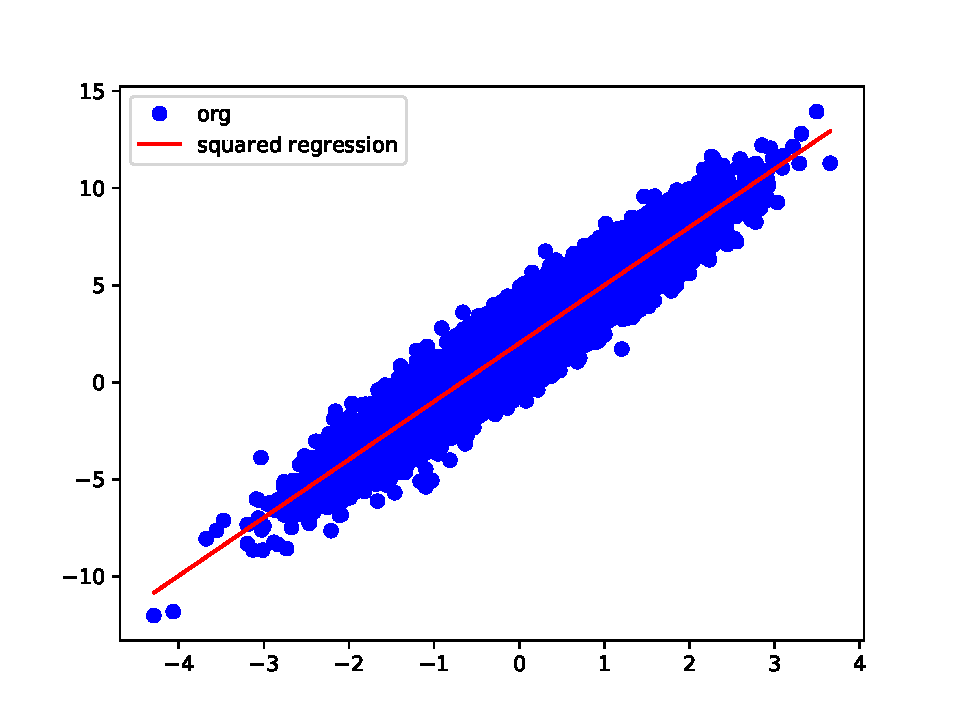
\includegraphics[scale=0.4]{imgs/squared.pdf}
  \end{minipage}
}
\quad
\quad
\subfigure[Huber loss]{
\begin{minipage}{0.4\linewidth}
\centering
  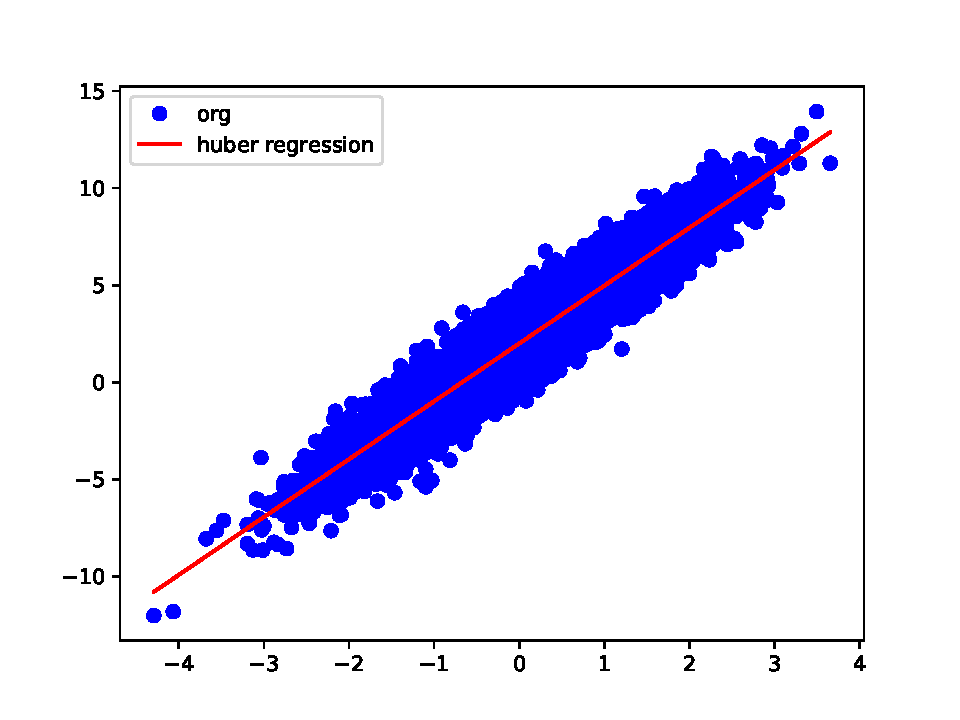
\includegraphics[scale=0.4]{imgs/huber.pdf}
  \end{minipage}
}


\subfigure[Hybrid loss]{
\begin{minipage}{0.4\linewidth}
\centering
  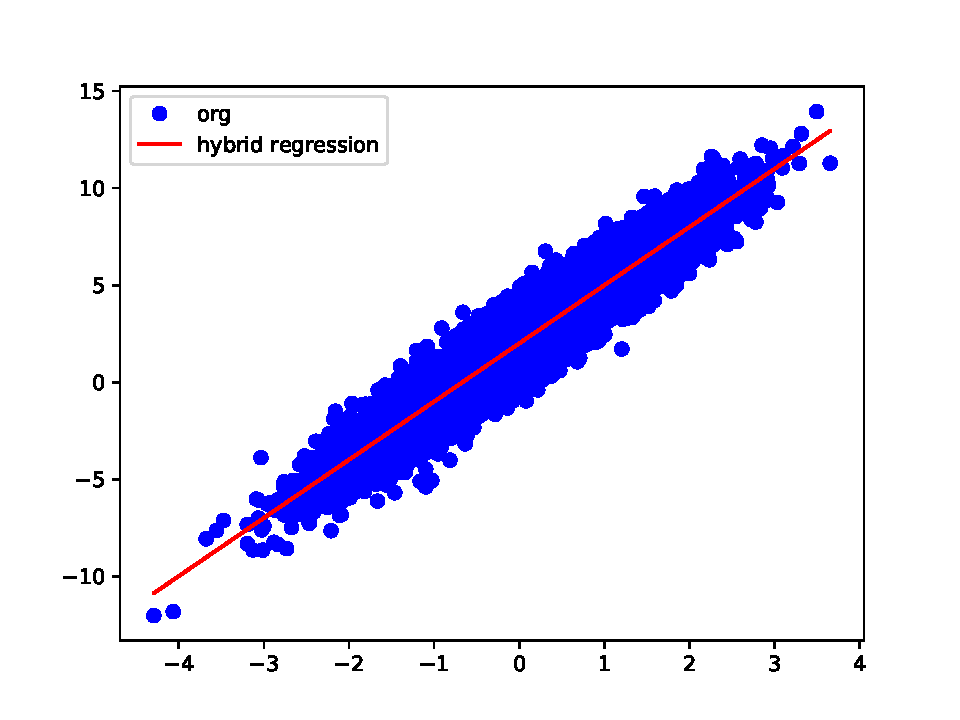
\includegraphics[scale=0.4]{imgs/hybrid.pdf}
  \end{minipage}
}
\quad
\quad
\subfigure[Performance of different loss function]{
\begin{minipage}{0.4\linewidth}
\centering
  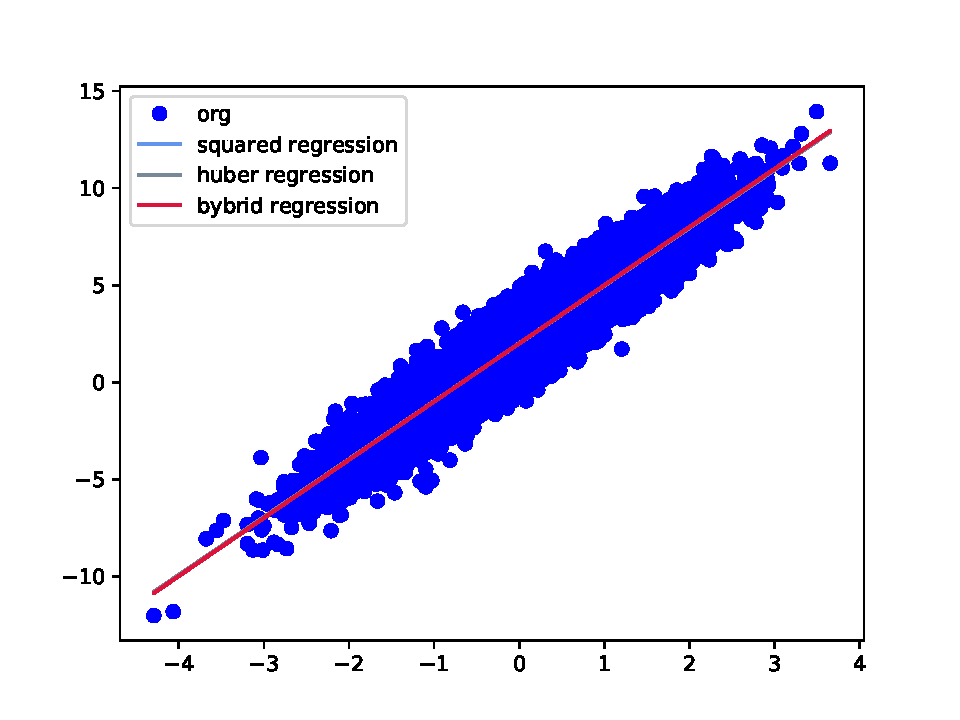
\includegraphics[scale=0.4]{imgs/all.pdf}
  \end{minipage}
}
\caption{ Loss function}
\label{loss}
\end{figure}

I also implement the following hybrid loss function and the performance shown in Figure \ref{loss} (c). 
$$hybrid\_loss = huber\_loss + |y - \hat{y}|$$

If I didn't use $tf.reduce\_mean$ in squared loss, the result of parameters $W$ and $b$ will turn out to be NaN. I found the issue will happen on TensorFlow 2.0. But on Tensorflow 1.14, sometimes it can output a correct answer. I'm not sure about the reason. But I think the loss is too large, which may result in NaN after several steps of gradients. 

It's hard to tell which loss function works better(see Figure\ref{loss} (d). I've run the code with those two loss functions multiple times and both of them work well. If I use the distance of the predicted parameters $\hat{W}, \hat{b}$ and original parameters $W, b$ as a measure of the performance($distances = |W-\hat{W}| + |b-\hat{b}|$), the squared loss(.0133321) work better than Huber loss(.0238144).


\subsection{Learning rate}

I implemented patience scheduling. Then I tested the learning rate from 0.001 to 0.01 with the incrementation 0.002, Shown in Figure \ref{lr}. Table \ref{tab:lr} shows the parameters learned under different learning rate with patience scheduling. The results are quite similar. All of them approximate to the correct parameters. 

\begin{figure}
  \centering
  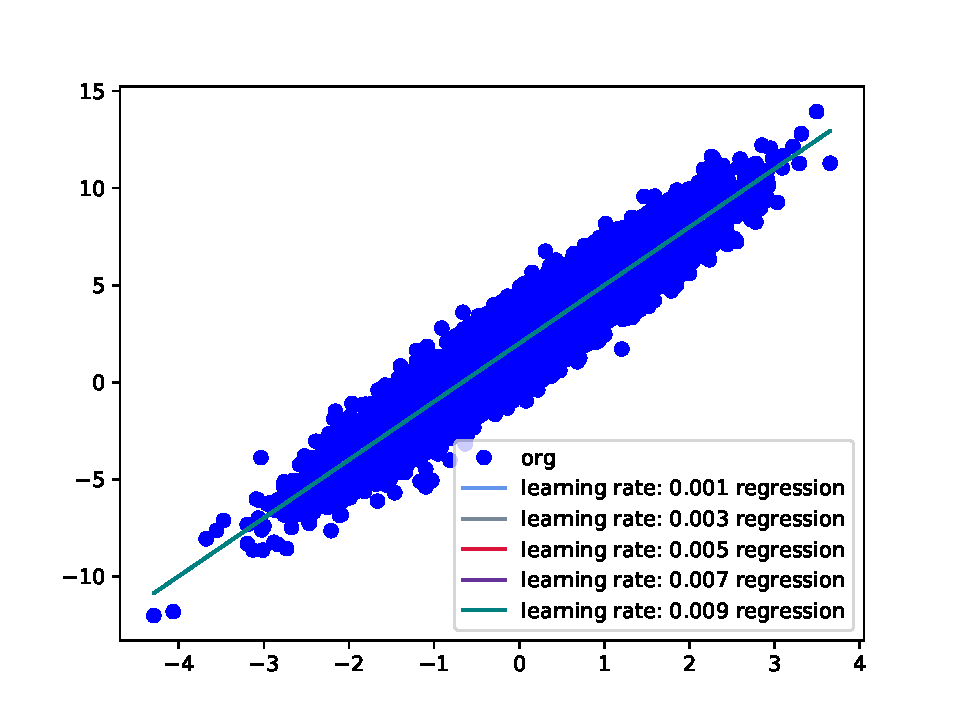
\includegraphics[scale=0.5]{imgs/lr.pdf}
  \caption{Learning rate}
  \label{lr}
\end{figure}

\begin{table}
  \caption{The performance of different learning rate}
  \label{tab:lr}
  \centering
  \begin{tabular}{lll}
    \toprule
    Learning rate     & W     & b \\
    \midrule
    0.001 & 2.9962702  & 2.0017185     \\
    0.003     & 2.9964287 & 2.001716     \\
    0.005     & 2.996503       & 2.0016577  \\
    0.007     & 2.996541 & 2.001543      \\
    0.009     & 2.9966085      & 2.0013998  \\
    \bottomrule
  \end{tabular}
\end{table}

\subsection{Training steps}
I've tested different training steps from 500 to 1500 with the incrementation 200. Shown in Figure \ref{ts}. With a longer duration, the performance tends to be better. However, after "enough" steps, this effects start to stabilize (see Table \ref{tab:ts}).


\begin{figure}[!h]
  \centering
  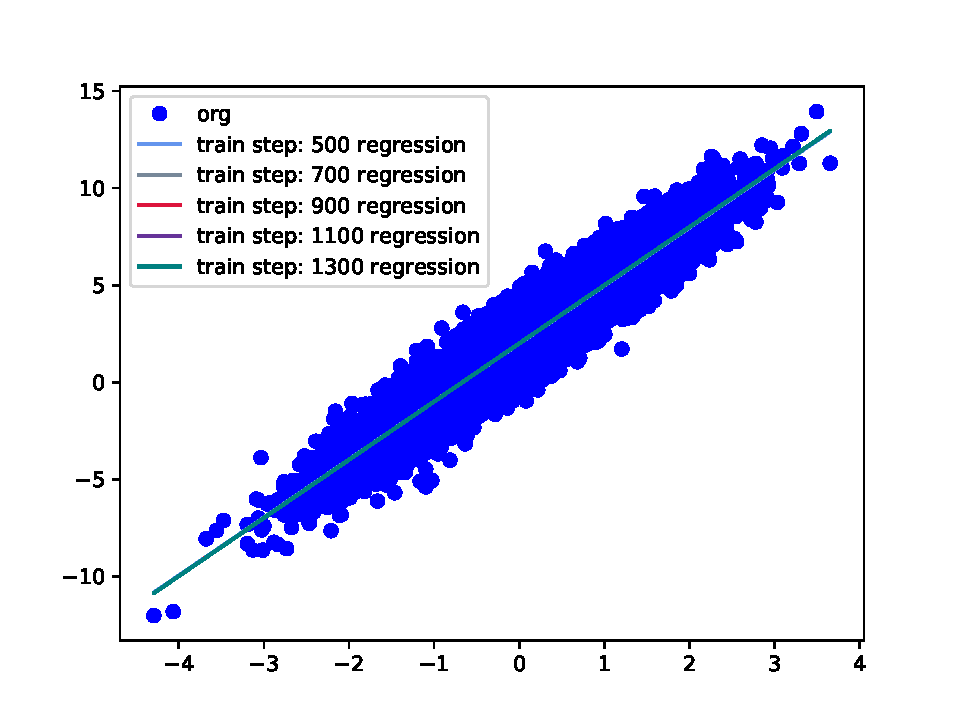
\includegraphics[scale=0.5]{imgs/ts.pdf}
  \caption{Training steps}
  \label{ts}
\end{figure}

\begin{table}[!h]
  \caption{The performance of different training steps}
  \label{tab:ts}
  \centering
  \begin{tabular}{lll}
    \toprule
    Training steps     & W     & b \\
    \midrule
    500 & 2.9877446  & 1.9952948     \\
    700     & 2.995941 & 2.001462     \\
    900     & 2.9962356       & 2.0016909  \\
    1100     & 2.9962835 & 2.001727      \\
    1300    & 2.9962983      & 2.0017405  \\
    \bottomrule
  \end{tabular}
\end{table}

\subsection{Initial Value of parameters}
Table \ref{tab:w} and Table \ref{tab:b} respectively denote predicted parameters with different initial parameter W and b(both of them are from -1000 to 1000 with the incrementation 500).

If I initialize the parameter W with a small number like -1000 with hybrid Loss, the predicted parameter W will become -984.0698 after 1000 epochs. That is because the model has not yet converged after 1000 epochs. Figure \ref{epoch} is the performance of different training epoch with the initial parameter $W=-100$. Despite the predicted parameters after 9000 epochs are far from the correct answer, it is gradually approaching to the correct answer.

\begin{table}[!h]
  \caption{The performance of different W after 1000 epochs}
  \label{tab:w}
  \centering
  \begin{tabular}{lll}
    \toprule
    Initial W     & W     & b  \\
    \midrule
    -1000 & -984.0698 & -0.16686472    \\
    -500     & -484.0088 & -0.12897438     \\
    0     & 2.9962702      & 2.0017185  \\
    500     & 484.0088 & 0.2609221     \\
    1000    & 984.0698     & 0.22580884  \\
    \bottomrule
  \end{tabular}
\end{table}

\begin{table}[!h]
  \caption{The performance of different b after 1000 epochs}
  \label{tab:b}
  \centering
  \begin{tabular}{lll}
    \toprule
    Initial b     & W     & b  \\
    \midrule
    -1000 & -0.19055721  & -979.8584     \\
    -500     & -0.19055721 & -479.8584     \\
    0     & 2.9962702       & 2.0017185  \\
    500     & 0.19055721 & 479.8584      \\
    1000    & 0.19055721     & 979.8584  \\
    \bottomrule
  \end{tabular}
\end{table}


\begin{figure}[!h]
  \centering
  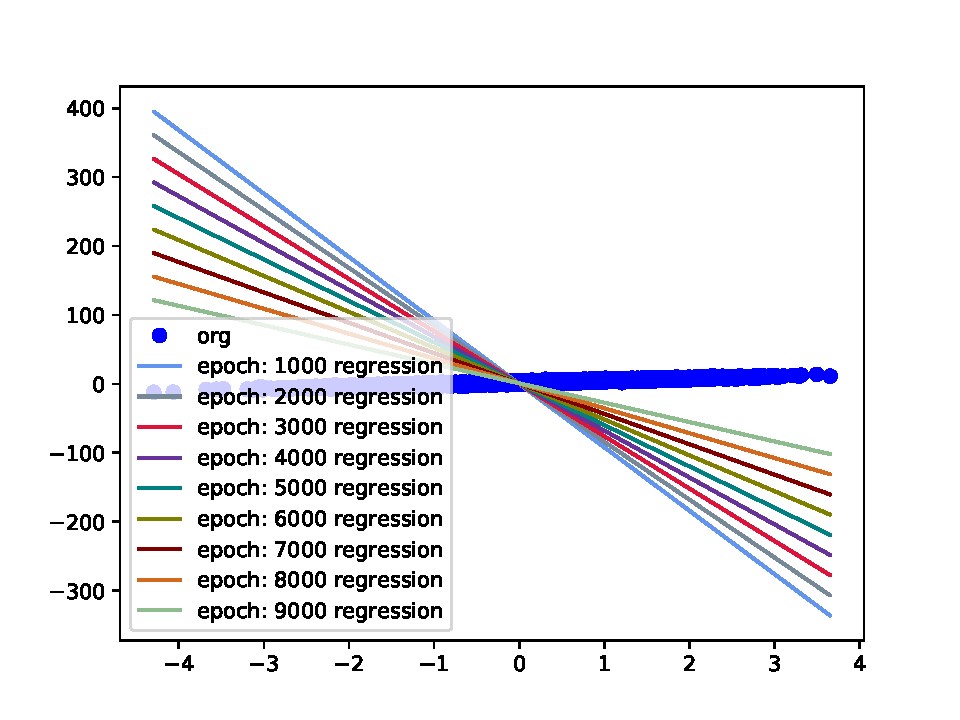
\includegraphics[scale=0.5]{imgs/epoch.pdf}
  \caption{Training duration with a large initiail parameter}
  \label{epoch}
\end{figure}

\subsection{Noise in data}
Before this section, I generated noise in data using the normal distribution. Table \ref{noise} shows the results of the different noise distribution. The distribution of noise can affect the prediction. Table \ref{normal1} shows the results of the normal distribution with different mean. Table \ref{normal2} shows the results of the normal distribution with different std. The level of noise is higher, the model is harder to converge.

\begin{table}[!h]
  \caption{The performance of different noise in data}
  \label{noise}
  \centering
  \begin{tabular}{lll}
    \toprule
    Noise distribution     & W     & b  \\
    \midrule
    normal(mean=0.0, stddev=1.0)     & 2.9794447 & 1.9967409    \\
    gamma(alpha=1)    & 2.98501      & 2.8410964  \\
    uniform(minval=0)    &2.9989622  &2.502729\\
    \bottomrule
  \end{tabular}
\end{table}

\begin{table}[!h]
  \caption{The performance of normal distribution with different mean}
  \label{normal1}
  \centering
  \begin{tabular}{lll}
    \toprule
    mean    & W     & b  \\
    \midrule
    0.0     & 2.9794447 & 1.9967409    \\
    1.0    & 2.964156 & 2.990973  \\
    2.0    &2.9483728 &3.9745786\\
    3.0    &2.924222 &4.9402742\\
    \bottomrule
  \end{tabular}
\end{table}

\begin{table}[!h]
  \caption{The performance of normal distribution with different std}
  \label{normal2}
  \centering
  \begin{tabular}{lll}
    \toprule
    mean    & W     & b  \\
    \midrule
    1.0    & 2.9794447 & 1.9967409 \\
    2.0    &2.8706882 &1.9283952\\
    3.0    &2.6891909 &1.8024324\\
    \bottomrule
  \end{tabular}
\end{table}

\subsection{Noise in data during training}
First, I tested adding noises(normal distribution: $mean = 0.$, $stddev=1.$) in data per epoch. The predicted parameters are $\hat{W }= 1.4970689$, $\hat{b}=1.8999192$.

Then, I added noises(normal distribution: $mean = 0.1$, $stddev=0.1$) in weights per epoch. The predicted parameters are $\hat{W} = -15.267623$, $\hat{b}=1.1710013$. 

Finally, I added noises(normal distribution: $mean = 0.001$, $stddev=0.002$) in learning rate per epoch. The predicted parameters are $\hat{W} = 2.9953077$, $\hat{b}=2.007313$. 

Noise in data and weight will change the performance of the model. If noise in learning rate is reasonable, it may affect training time. But it will not change the general performance of the model, except it reaches local minima. For example, it may lead to faster convergence or make the model hard to converge. 

On other classification problems and mathematical models, noise in data and weight will also reduce the model's performance. But adding small noise in learning rate may make it possible to get rid of local minima.  

\subsection{Significance of seed}
If I use the same seed to generate noise, I will get the same results every time I run the code without change any parameters. Because the pseudorandom number generating algorithms is designed for performing an operation on a seed. So the result of algorithms is determined by the seed. If I want to change the result every time, I can use the current time as the seed.

%\subsection{Dropout}
%On real-world dataset, I'll try to dropout some values because usually, the outliers are not 

\subsection{GPU VS CPU}
I tested training time with GPU and CPU on Calab. I used each of them to run the same code for 1000 epochs. And the approximate running time of CPU per epoch is 0.029198 and of GPU is 0.05428. 

The training time looks unreasonable. I think it may be because it's not the correct running time considering the network speed and the design of Calab. It may also because the linear regression model doesn't fit to calculate on GPU.

\section{Problem 2}
Solved on 09/21/2019. 

\subsection{Performance of three models}
I implemented three models for fminist. 

The first one is Vgg16(shown as Figure \ref{vgg}). Another one is multilayer CNNs with batch norm. The accuracy of Vgg16 on test dataset can achieve 92.45\% after 15 epochs. 
\begin{figure}[!h]
  \centering
  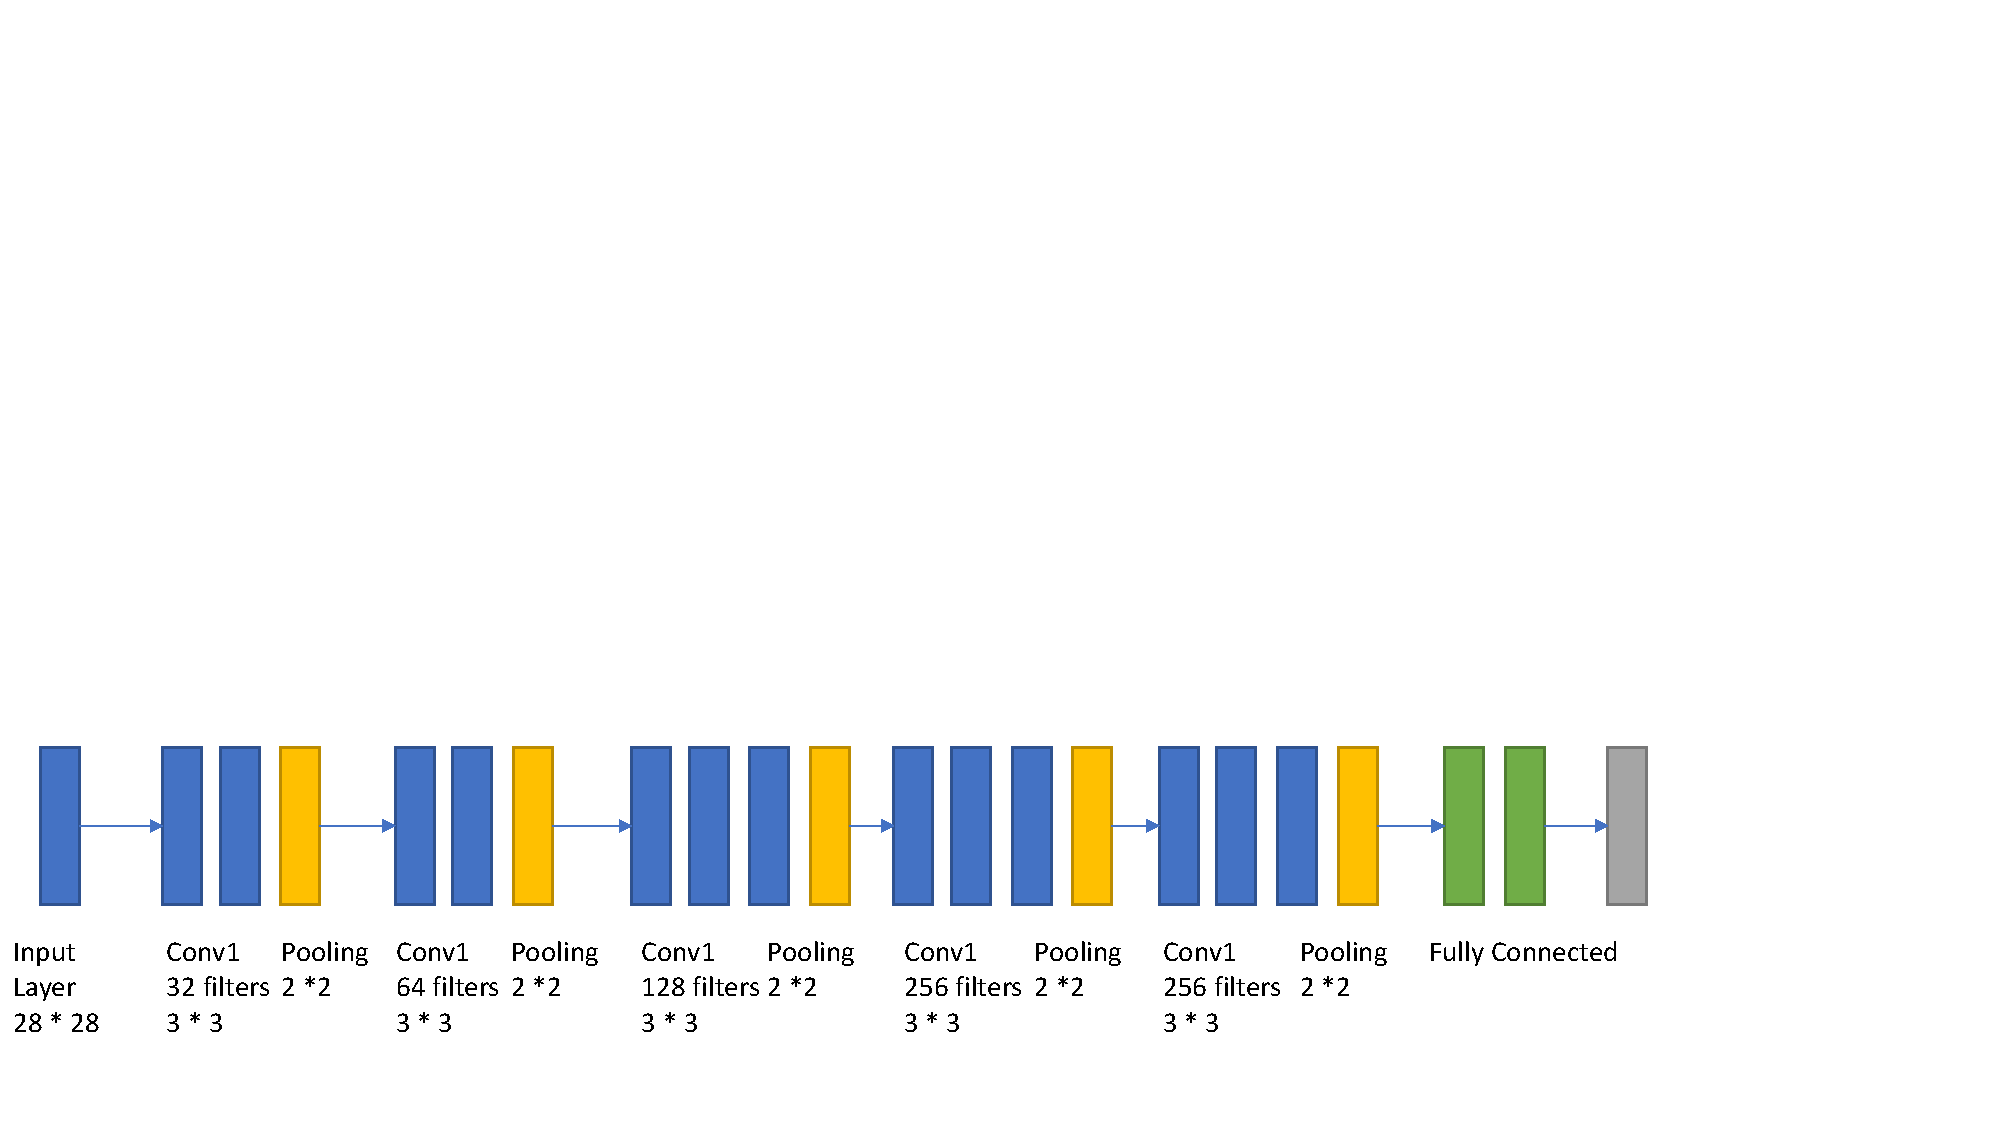
\includegraphics[scale=0.5]{imgs/vgg.pdf}
  \caption{Vgg16}
  \label{vgg}
\end{figure}

Another model achieves 90.67\% after 120 epochs. Figure \ref{res} is an example of images and CNNs model's prediction. Figure \ref{filt} is the weights of the first layer in CNNs model. 
\begin{figure}[!h]
  \centering
  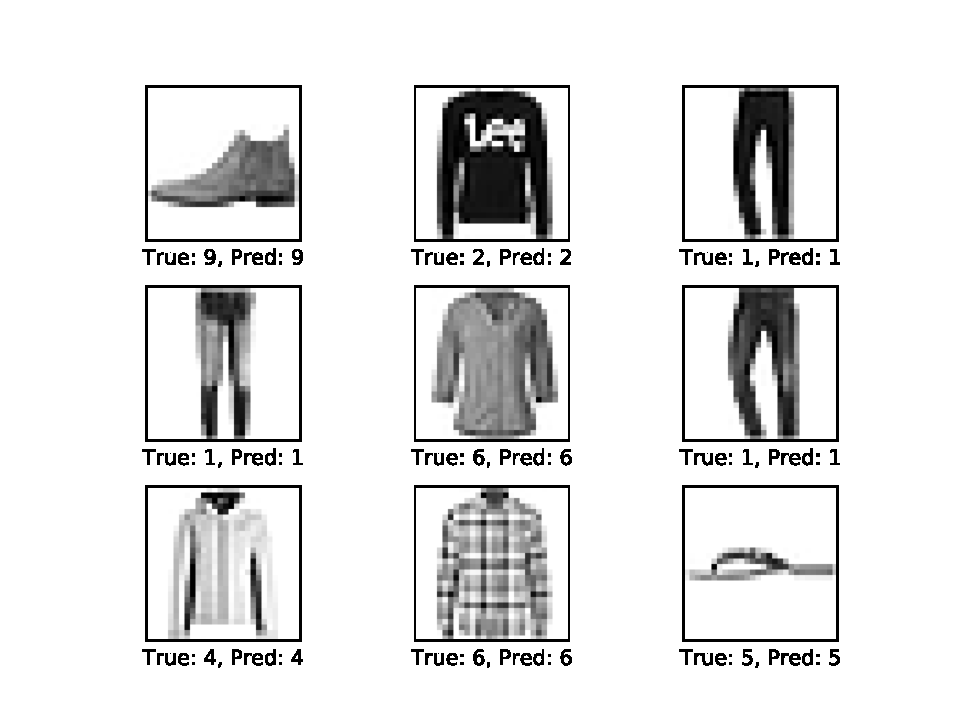
\includegraphics[scale=0.4]{imgs/result.pdf}
  \caption{Samples}
  \label{res}
\end{figure}

\begin{figure}[!h]
  \centering
  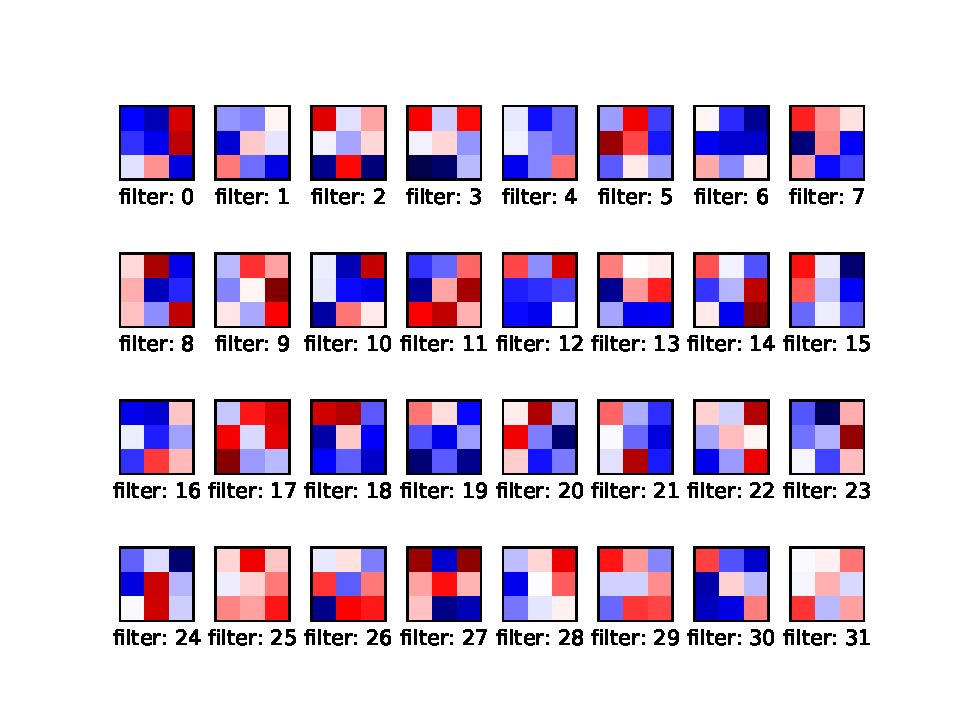
\includegraphics[scale=0.5]{imgs/weight.pdf}
  \caption{Filters' weights of the first layer in CNNs model}
  \label{filt}
\end{figure}

I also implement linear model as problem 1 in this dataset. It can achieve 82.6\% after 120 epochs. Figure \ref{weight} is the weights of the first layer in CNNs model.

\begin{figure}[!h]
  \centering
  \includegraphics[scale=1.]{imgs/weights.pdf}
  \caption{Weights of the first layer in linear model}
  \label{weight}
\end{figure}

The following reports are based on multilayer CNNs model not Vgg16, because Vgg16 takes for a while per epoch.


\subsection{Optimizer}
Figure \ref{adam} is the loss and accuracy of train dataset and test dataset using Adam optimizer. Figure \ref{ada} is the performance of Adagrad optimizer. Figure\ref{nadam} is the performance of Nadam optimizer. Adam optimizer could converge faster and generalize better. I tested SGD Optimizer($momentum=0.9$). After 8 iterations, the loss will turn to $NaN$. Maybe it is the same reason I listed in problem 1. The exploding gradients problem lead to overflow at some point during gradient descent and cause NaNs.

\begin{figure}[!h]
\subfigure[train loss ]{
  \begin{minipage}{0.21\linewidth}
  \centering
  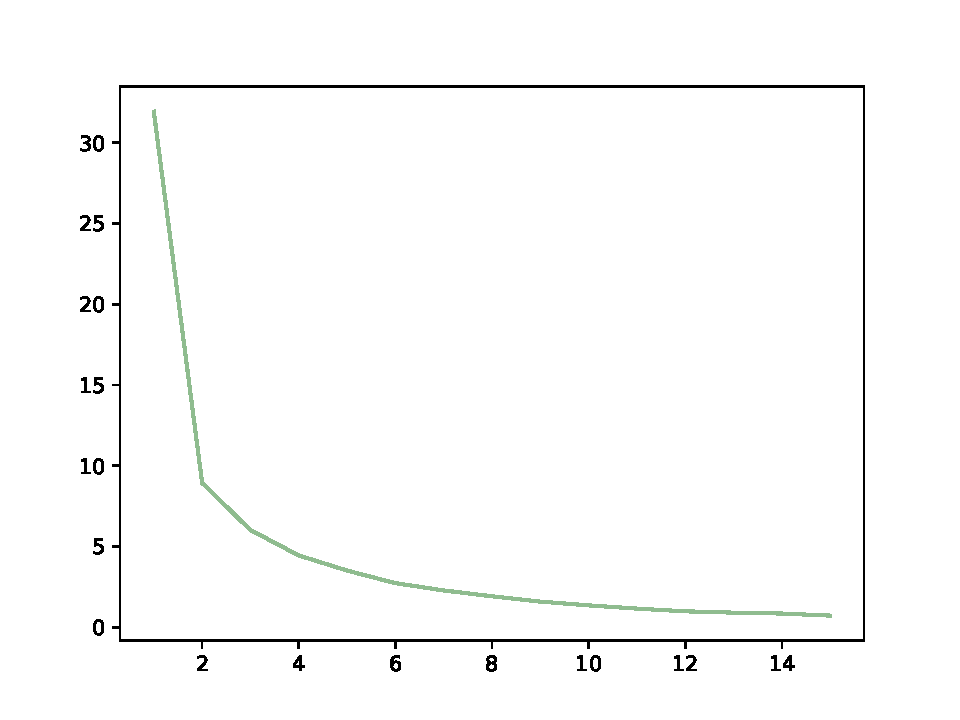
\includegraphics[scale=0.23]{imgs/train_loss_adam.pdf}
  \end{minipage}
}
\quad
\subfigure[train accuracy ]{
\begin{minipage}{0.21\linewidth}
\centering
  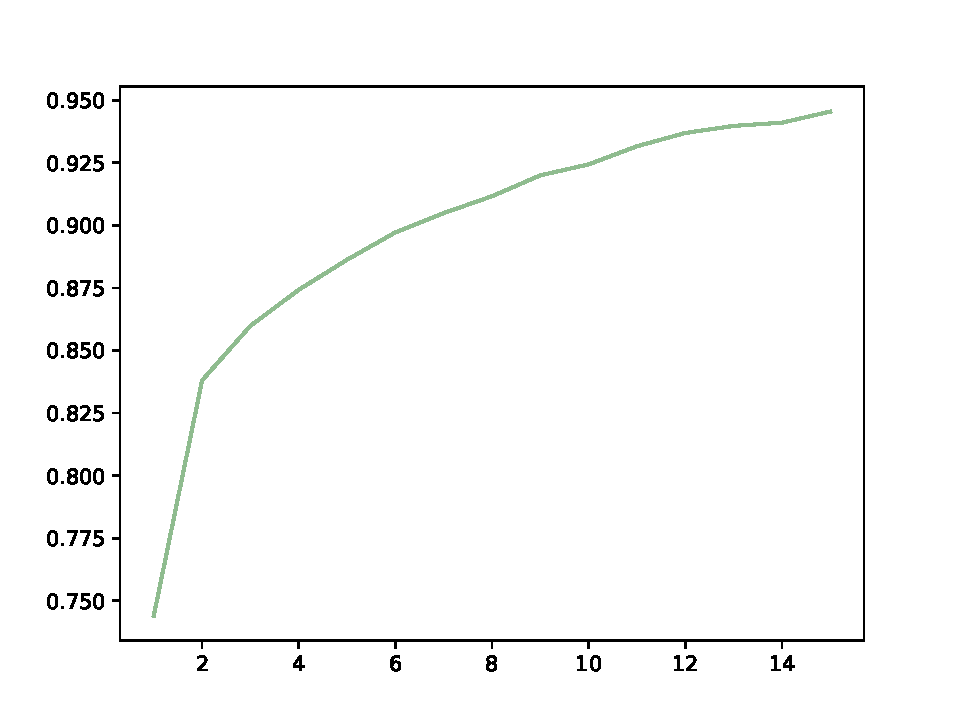
\includegraphics[scale=0.23]{imgs/train_acc_adam.pdf}
  \end{minipage}
}
\quad
\subfigure[test loss ]{
\begin{minipage}{0.21\linewidth}
\centering
  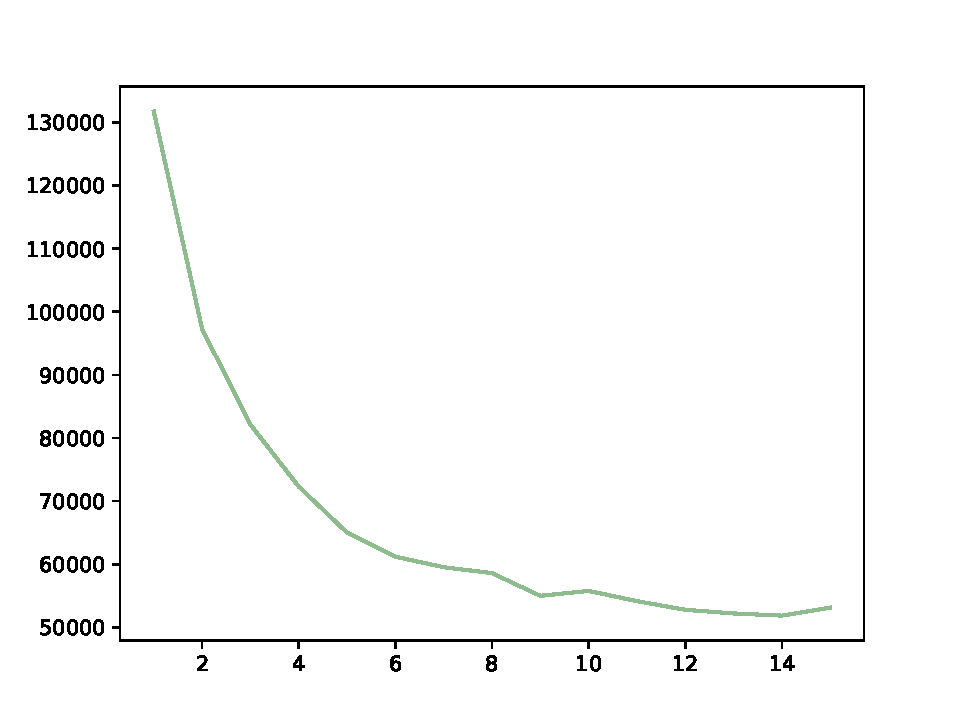
\includegraphics[scale=0.23]{imgs/test_loss_adam.pdf}
  \end{minipage}
}
\quad
\subfigure[test accuracy ]{
\begin{minipage}{0.21\linewidth}
\centering
  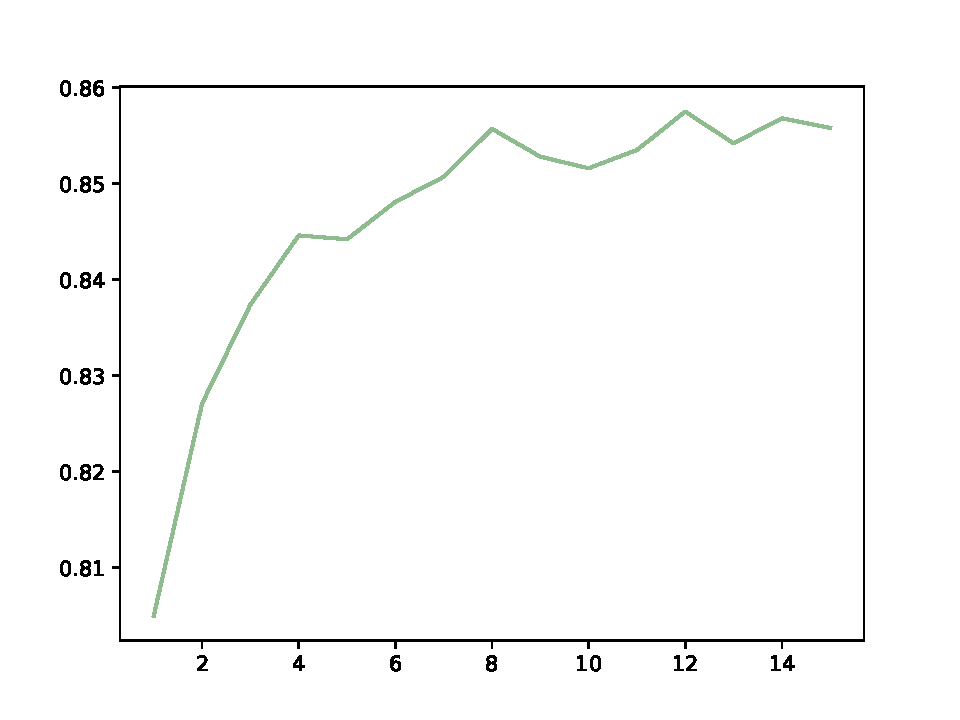
\includegraphics[scale=0.23]{imgs/test_acc_adam.pdf}
  \end{minipage}
}
\caption{ Adam Optimizer}
\label{adam}
\end{figure}

\begin{figure}[!h]
\subfigure[train loss]{
  \begin{minipage}{0.21\linewidth}
  \centering
  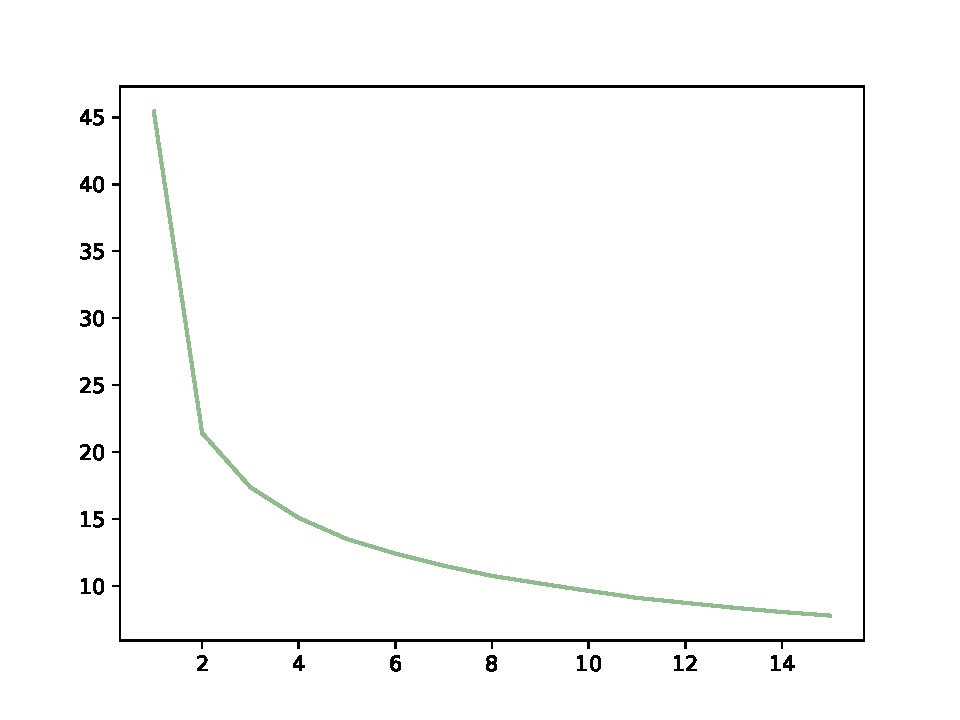
\includegraphics[scale=0.23]{imgs/train_loss_ada.pdf}
  \end{minipage}
}
\quad
\subfigure[train accuracy ]{
\begin{minipage}{0.21\linewidth}
\centering
  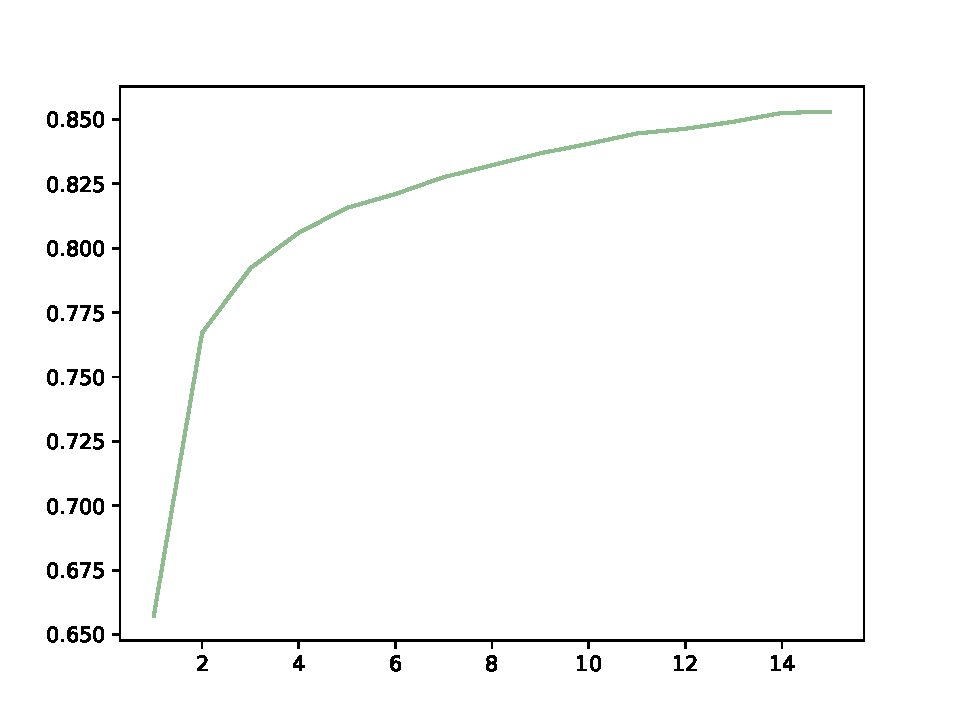
\includegraphics[scale=0.23]{imgs/train_acc_ada.pdf}
  \end{minipage}
}
\quad
\subfigure[test loss ]{
\begin{minipage}{0.21\linewidth}
\centering
  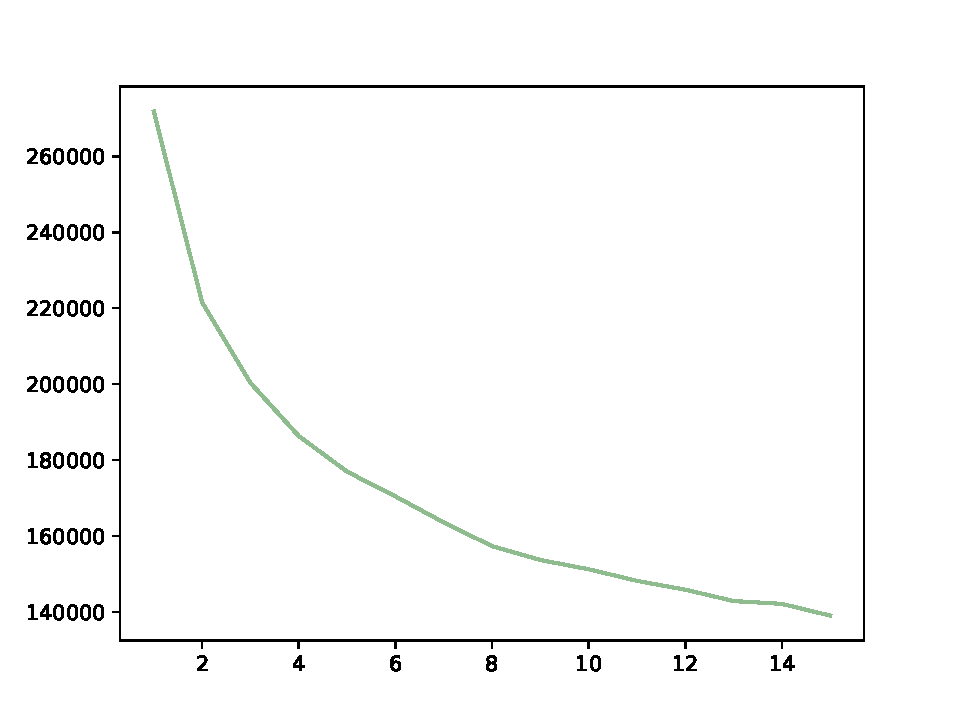
\includegraphics[scale=0.23]{imgs/test_loss_ada.pdf}
  \end{minipage}
}
\quad
\subfigure[test accuracy ]{
\begin{minipage}{0.21\linewidth}
\centering
  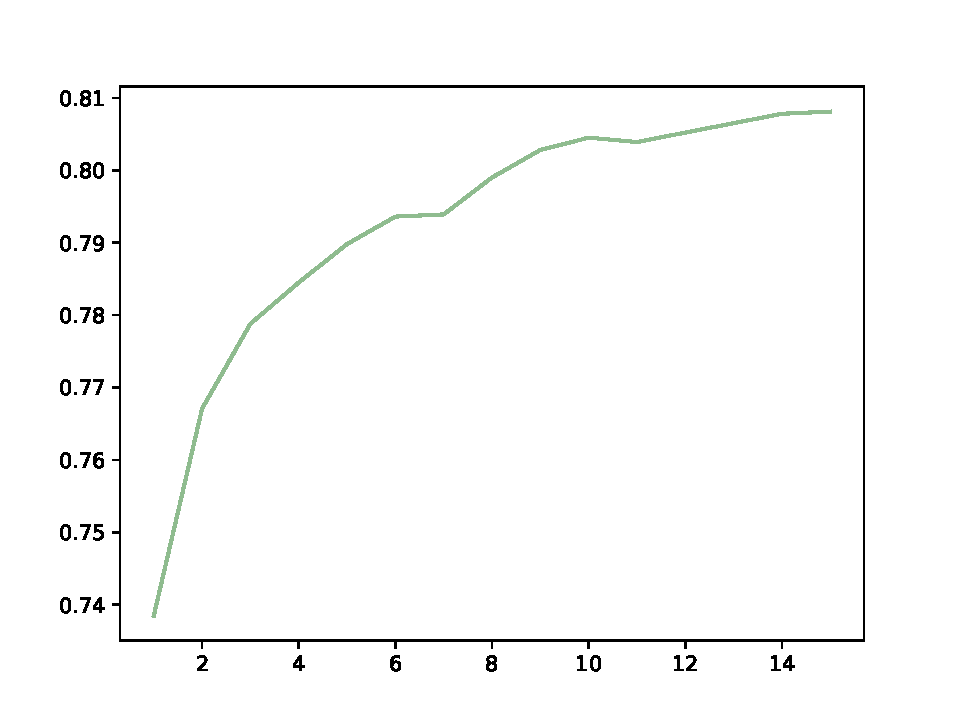
\includegraphics[scale=0.23]{imgs/test_acc_ada.pdf}
  \end{minipage}
}
\caption{ Adagrad Optimizer}
\label{ada}
\end{figure}


\begin{figure}[!h]
\subfigure[train loss ]{
  \begin{minipage}{0.21\linewidth}
  \centering
  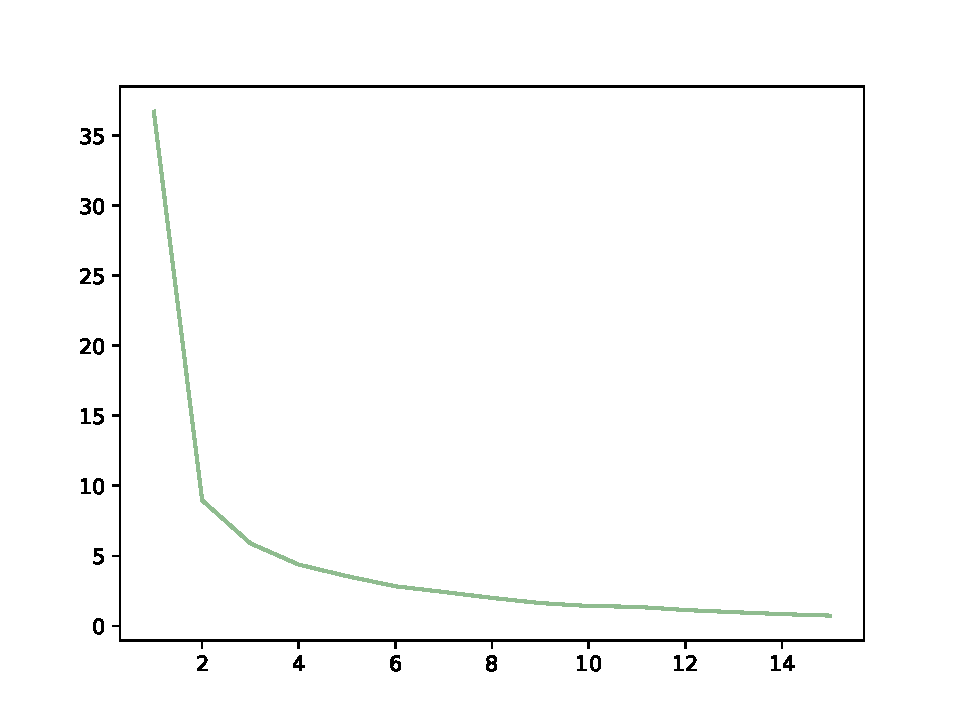
\includegraphics[scale=0.23]{imgs/train_loss_nadam.pdf}
  \end{minipage}
}
\quad
\subfigure[train accuracy ]{
\begin{minipage}{0.21\linewidth}
\centering
  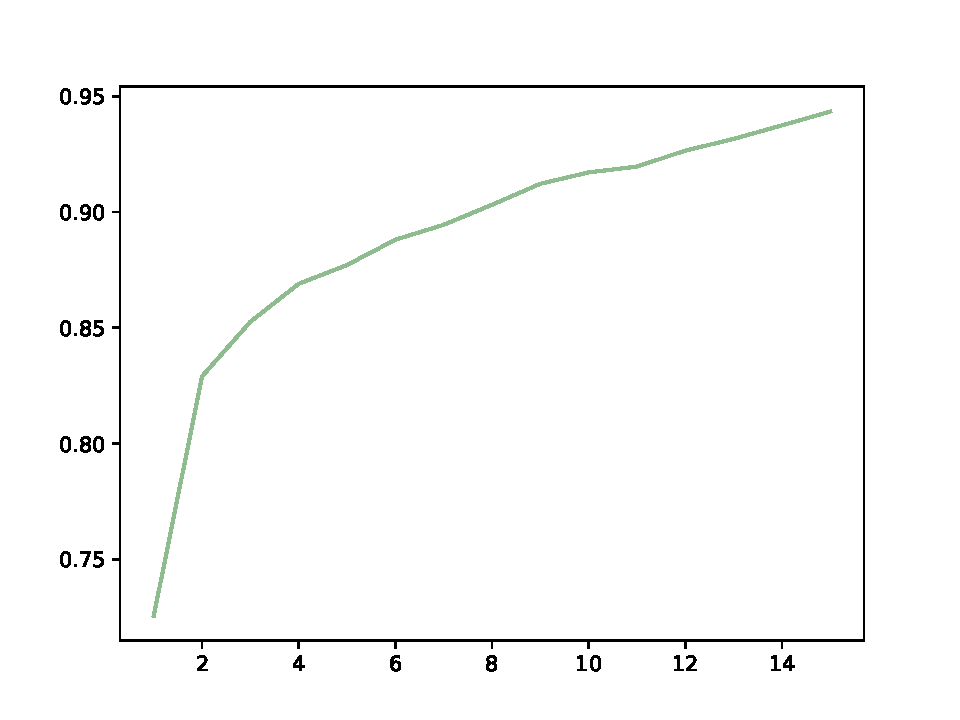
\includegraphics[scale=0.23]{imgs/train_acc_nadam.pdf}
  \end{minipage}
}
\quad
\subfigure[test loss ]{
\begin{minipage}{0.21\linewidth}
\centering
  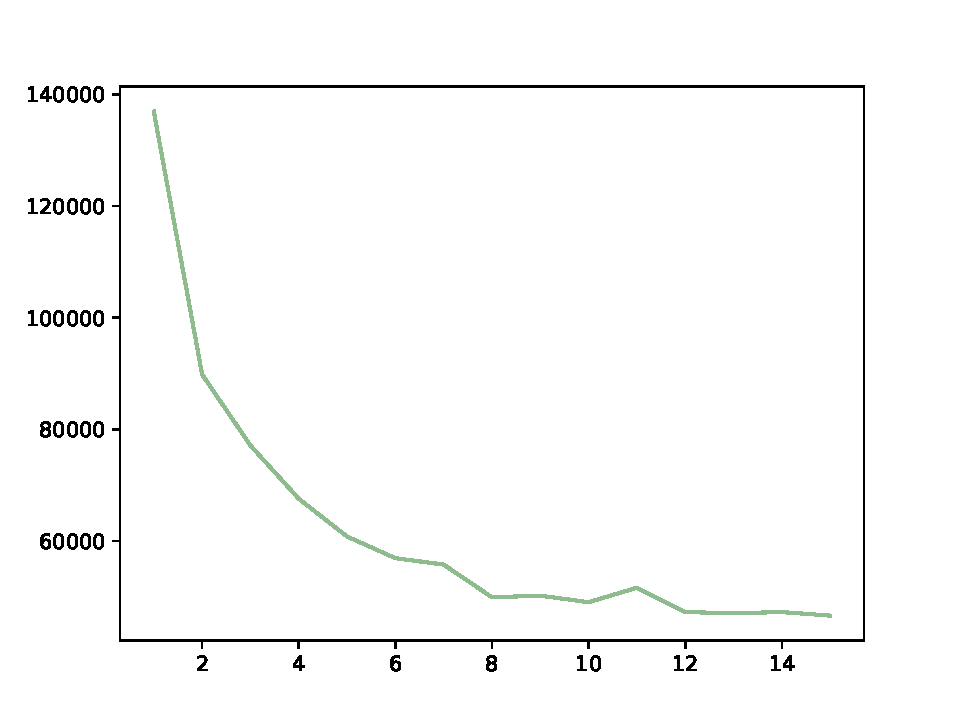
\includegraphics[scale=0.23]{imgs/test_loss_nadam.pdf}
  \end{minipage}
}
\quad
\subfigure[test accuracy ]{
\begin{minipage}{0.21\linewidth}
\centering
  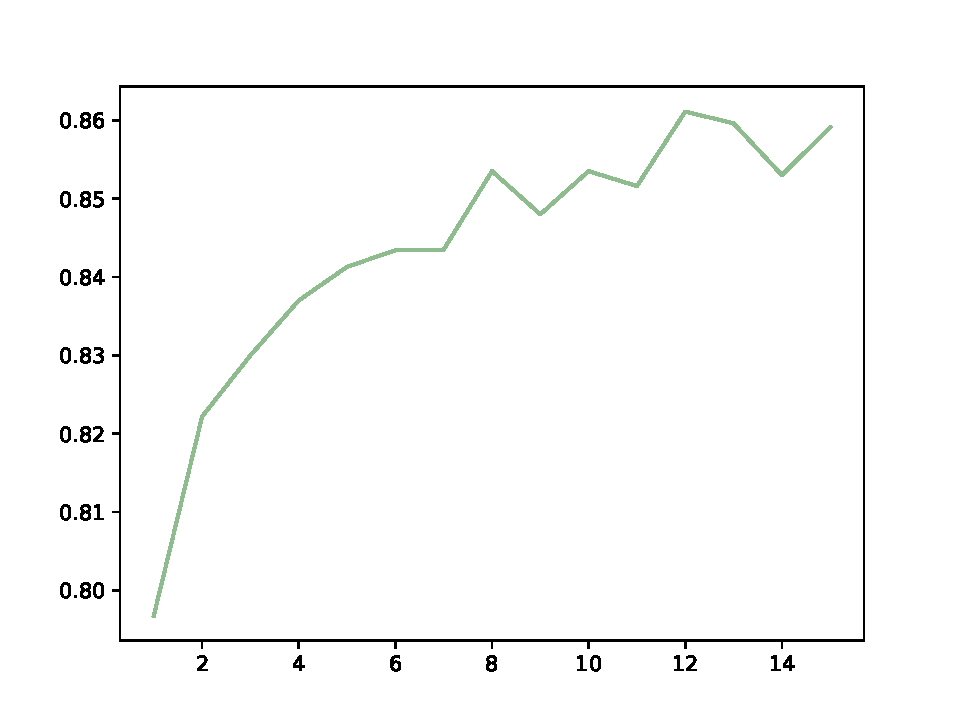
\includegraphics[scale=0.23]{imgs/test_acc_nadam.pdf}
  \end{minipage}
}
\caption{ NAdam Optimizer}
\label{nadam}
\end{figure}

\subsection{Train for longer epochs}
Figure \ref{over} is the result if I train the model for more epochs. At first, I thought the decreasing accuracy on test dataset means the model is already overfitting. But with longer epochs, it turns out the model just fall into local minima. And the accuracy can reach 90.67\% after 120 epochs.

Figure \ref{vgg16} is the result if I train the Vgg model for more epochs. This model is better than CNNs because it can converge faster and generalize better. After 20 epochs, it has gotten a stable result. It can get achieve 93.26\% within 120 epochs.

\begin{figure}[!h]
\subfigure[train loss ]{
  \begin{minipage}{0.21\linewidth}
  \centering
  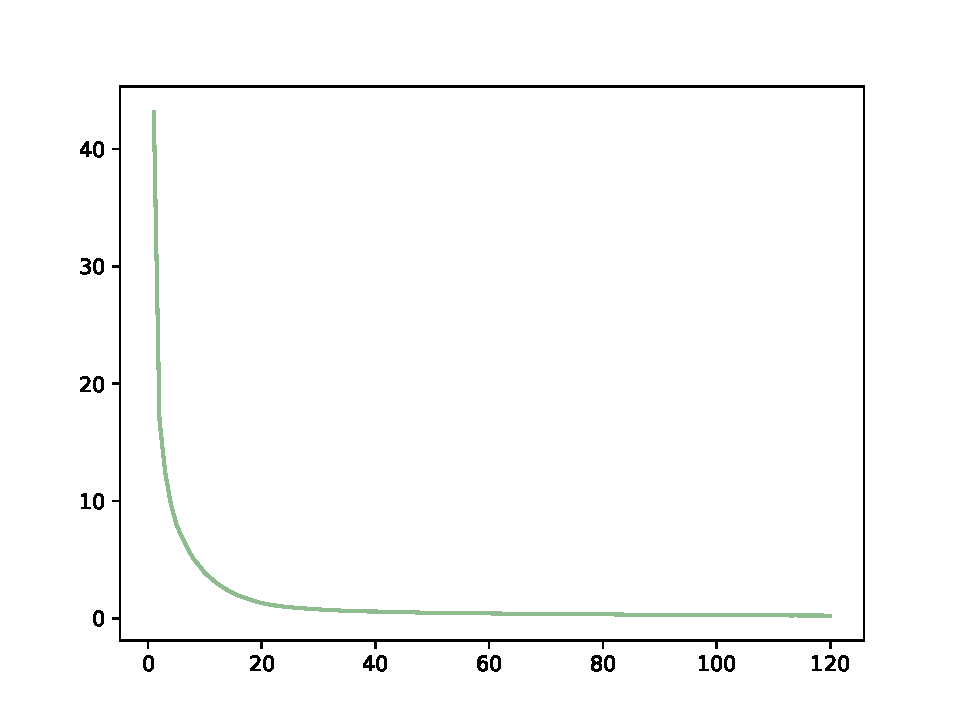
\includegraphics[scale=0.23]{imgs/train_loss_fit.pdf}
  \end{minipage}
}
\quad
\subfigure[train accuracy ]{
\begin{minipage}{0.21\linewidth}
\centering
  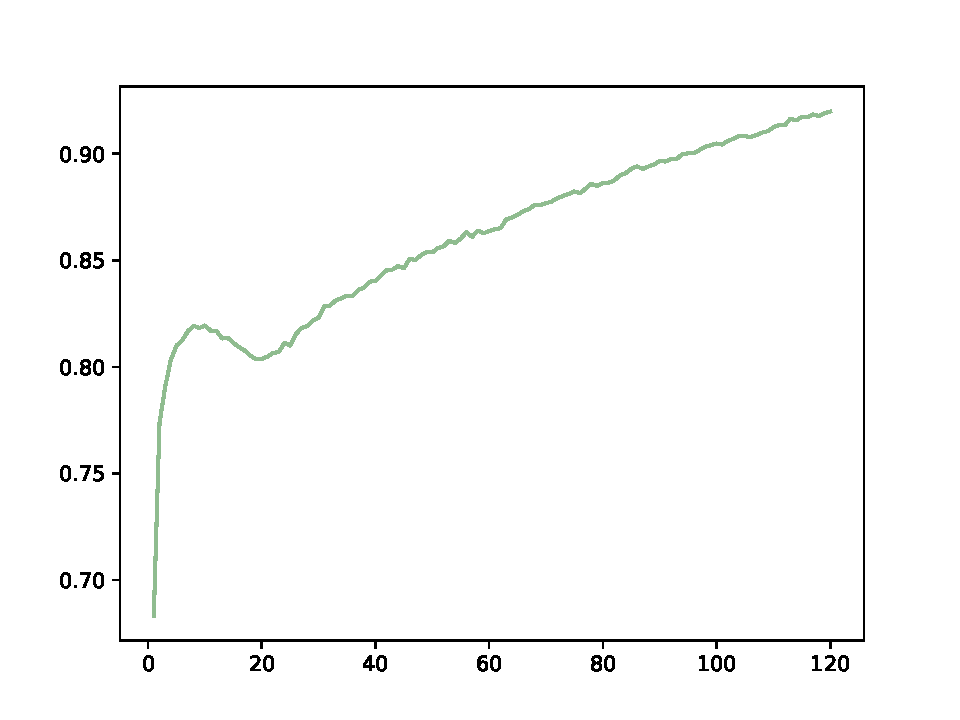
\includegraphics[scale=0.23]{imgs/train_acc_fit.pdf}
  \end{minipage}
}
\quad
\subfigure[test loss ]{
\begin{minipage}{0.21\linewidth}
\centering
  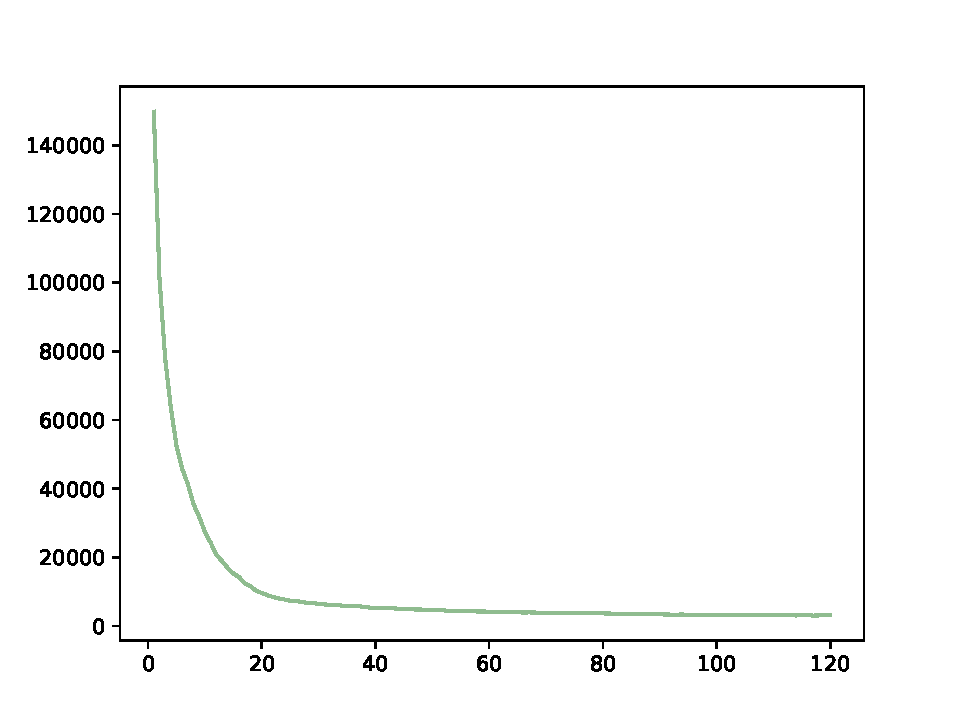
\includegraphics[scale=0.23]{imgs/test_loss_fit.pdf}
  \end{minipage}
}
\quad
\subfigure[test accuracy ]{
\begin{minipage}{0.21\linewidth}
\centering
  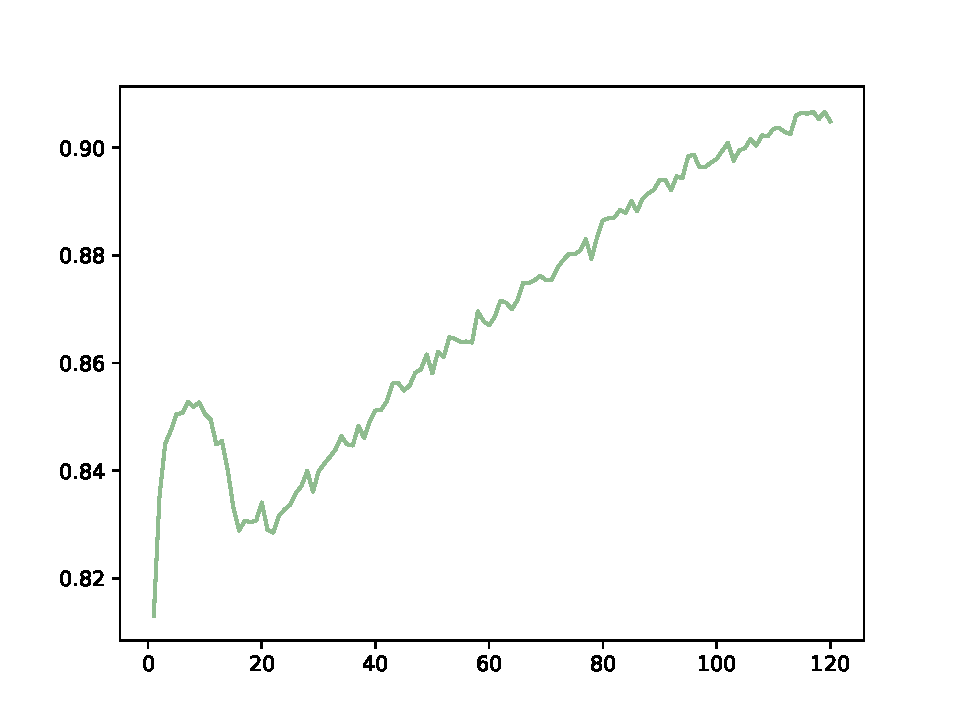
\includegraphics[scale=0.23]{imgs/test_acc_fit.pdf}
  \end{minipage}
}
\caption{More Training time}
\label{over}
\end{figure}

\begin{figure}[!h]
\subfigure[train loss ]{
  \begin{minipage}{0.21\linewidth}
  \centering
  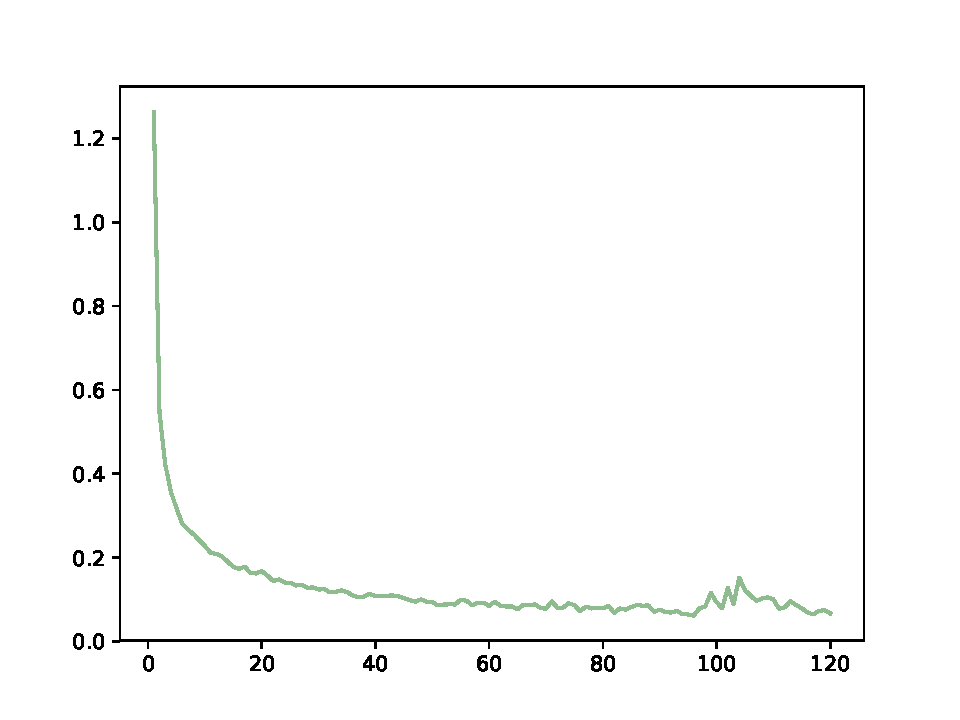
\includegraphics[scale=0.23]{imgs/train_loss_vgg.pdf}
  \end{minipage}
}
\quad
\subfigure[train accuracy ]{
\begin{minipage}{0.21\linewidth}
\centering
  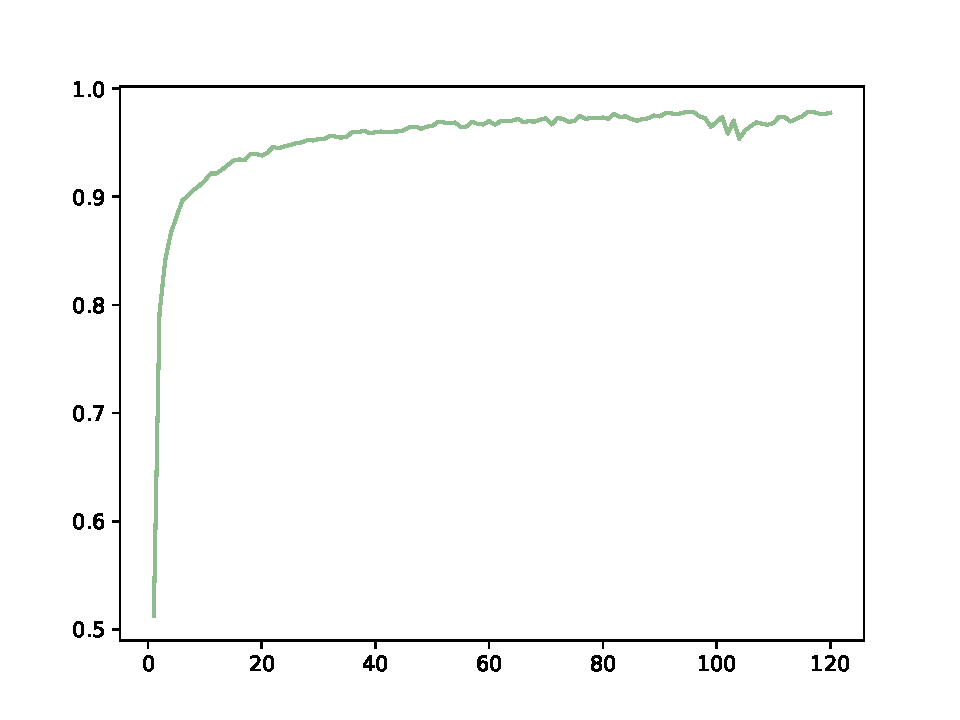
\includegraphics[scale=0.23]{imgs/train_acc_vgg.pdf}
  \end{minipage}
}
\quad
\subfigure[test loss ]{
\begin{minipage}{0.21\linewidth}
\centering
  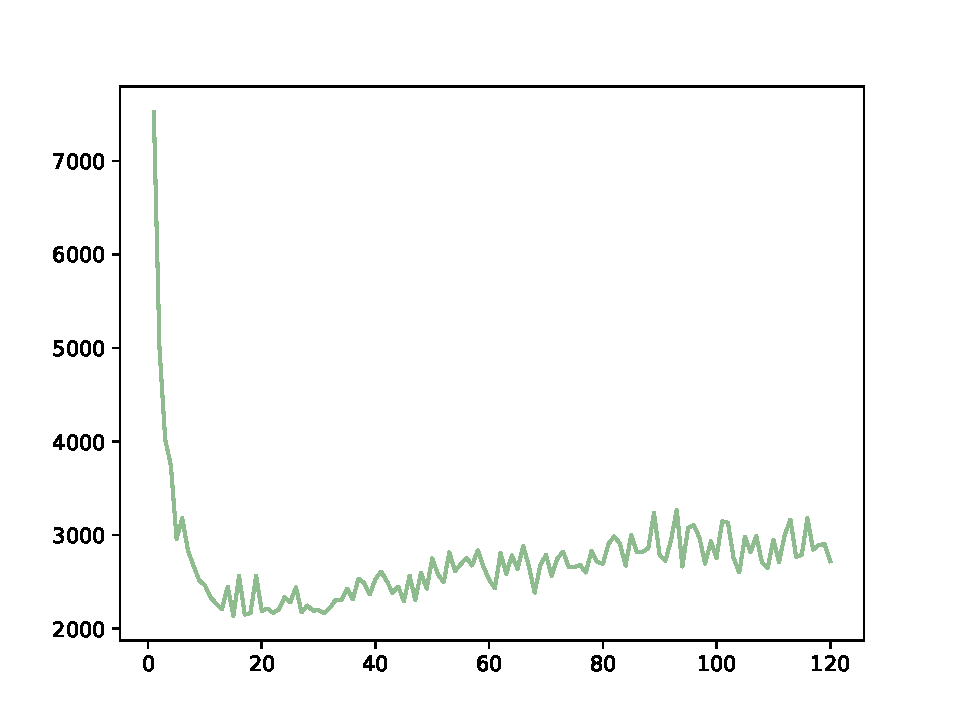
\includegraphics[scale=0.23]{imgs/test_loss_vgg.pdf}
  \end{minipage}
}
\quad
\subfigure[test accuracy ]{
\begin{minipage}{0.21\linewidth}
\centering
  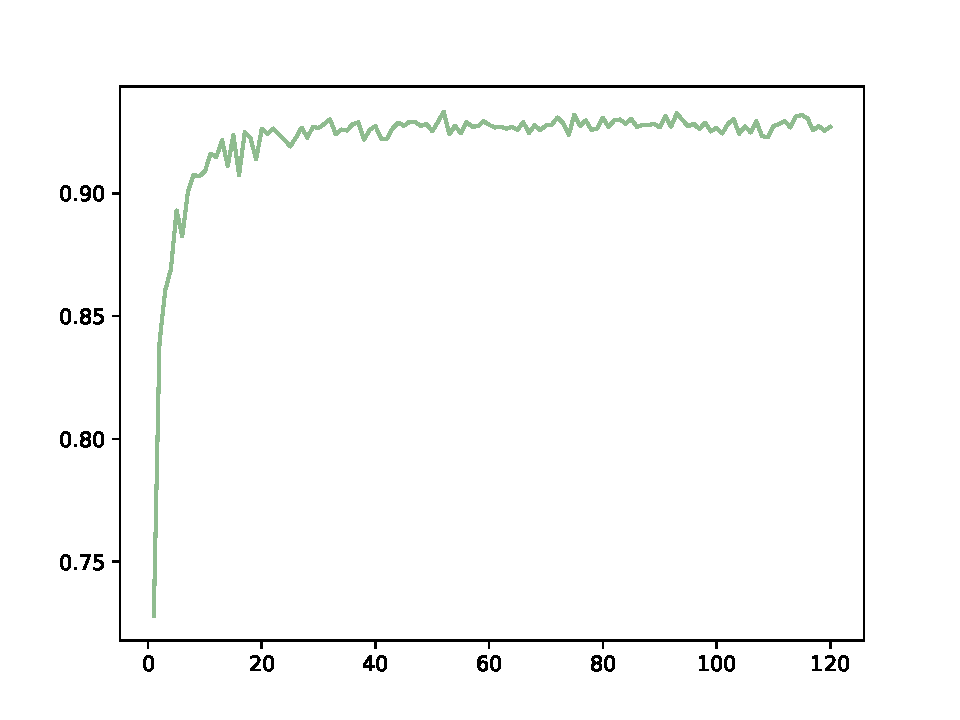
\includegraphics[scale=0.23]{imgs/test_acc_vgg.pdf}
  \end{minipage}
}
\caption{More Training time(VGG16)}
\label{vgg16}
\end{figure}

\subsection{Train/Val Split}
Figure \ref{tv0.1} is the result(best accuracy is 86.57\% on test dataset) that the proportion of train dataset to test dataset is 9:1. Before this section, the ratio of train and test dataset is 6:1, and the result(best accuracy on the test dataset is 85.87\%) shows in Figure \ref{adam}. Figure \ref{tv0.3} is the result(best accuracy is 86.10\% on test dataset) that the proportion of train dataset to test dataset is 7:3.   Figure \ref{tv0.4} is the result(best accuracy is 84.72\% on test dataset) that the proportion of train dataset to test dataset is 6:4. 

The model needs enough data to train, so less train dataset has greater variance. But more train dataset can not guarantee a robust measure of error.

\begin{figure}[!h]
\subfigure[train loss ]{
  \begin{minipage}{0.21\linewidth}
  \centering
  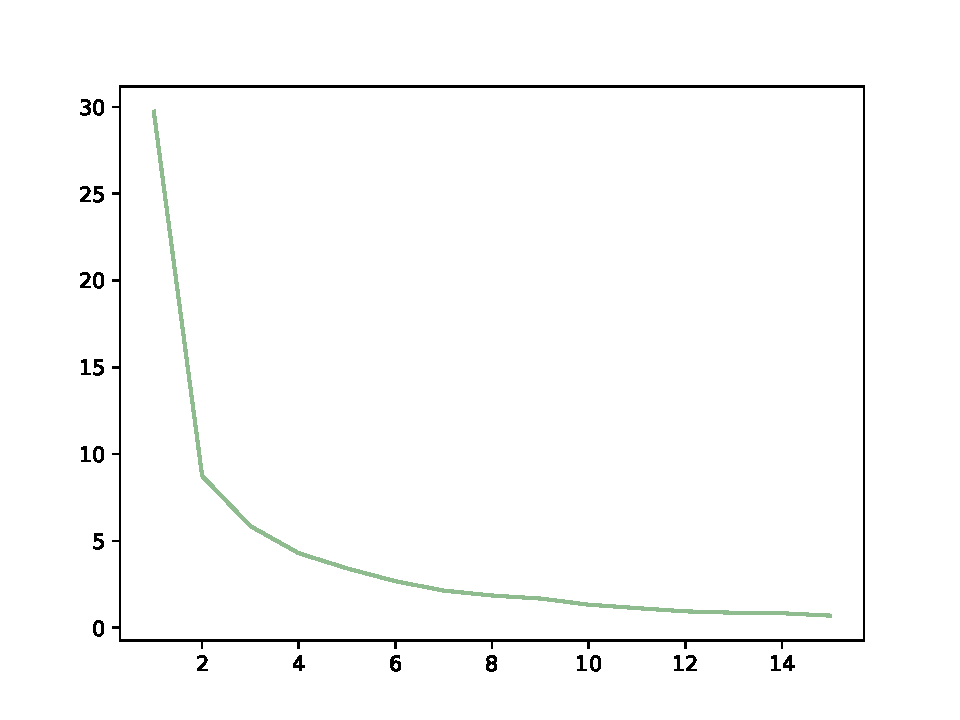
\includegraphics[scale=0.23]{imgs/train_loss_1.pdf}
  \end{minipage}
}
\quad
\subfigure[train accuracy ]{
\begin{minipage}{0.21\linewidth}
\centering
  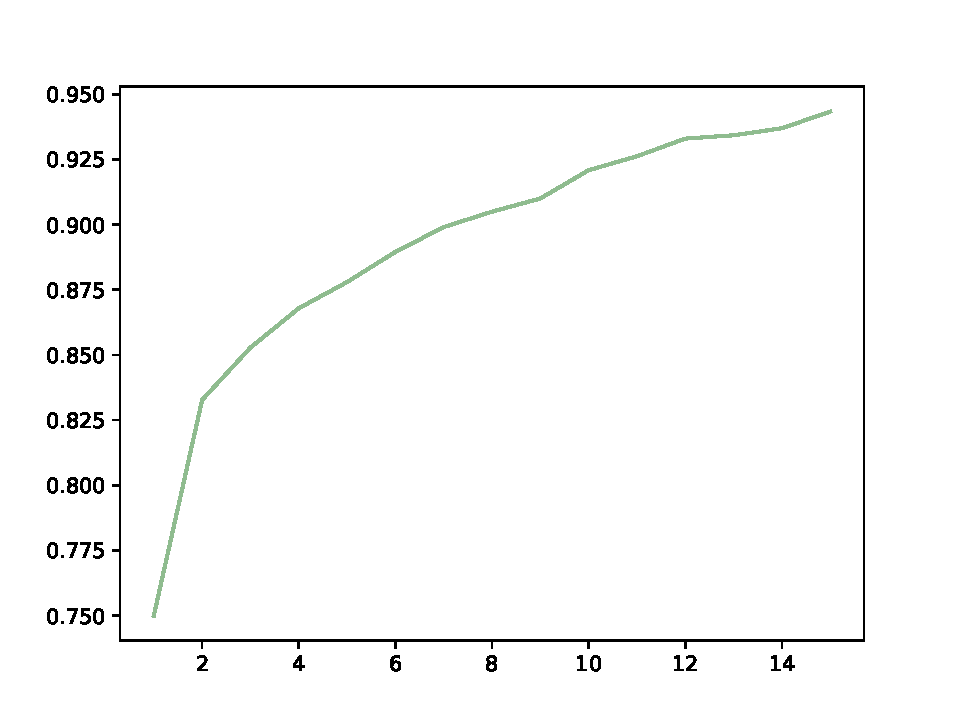
\includegraphics[scale=0.23]{imgs/train_acc_1.pdf}
  \end{minipage}
}
\quad
\subfigure[test loss ]{
\begin{minipage}{0.21\linewidth}
\centering
  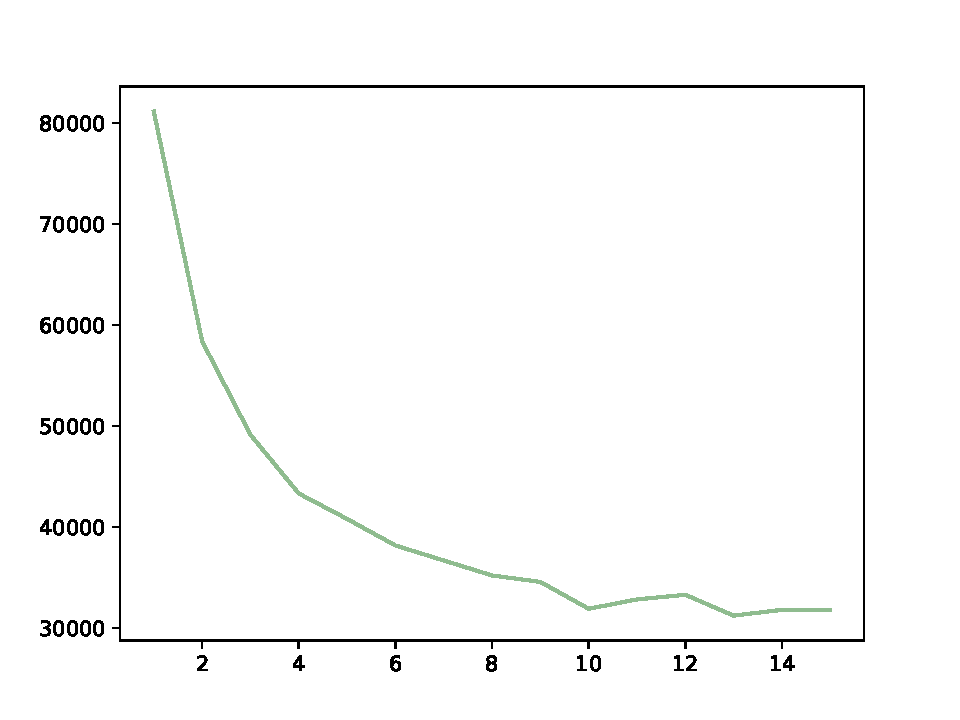
\includegraphics[scale=0.23]{imgs/test_loss_1.pdf}
  \end{minipage}
}
\quad
\subfigure[test accuracy ]{
\begin{minipage}{0.21\linewidth}
\centering
  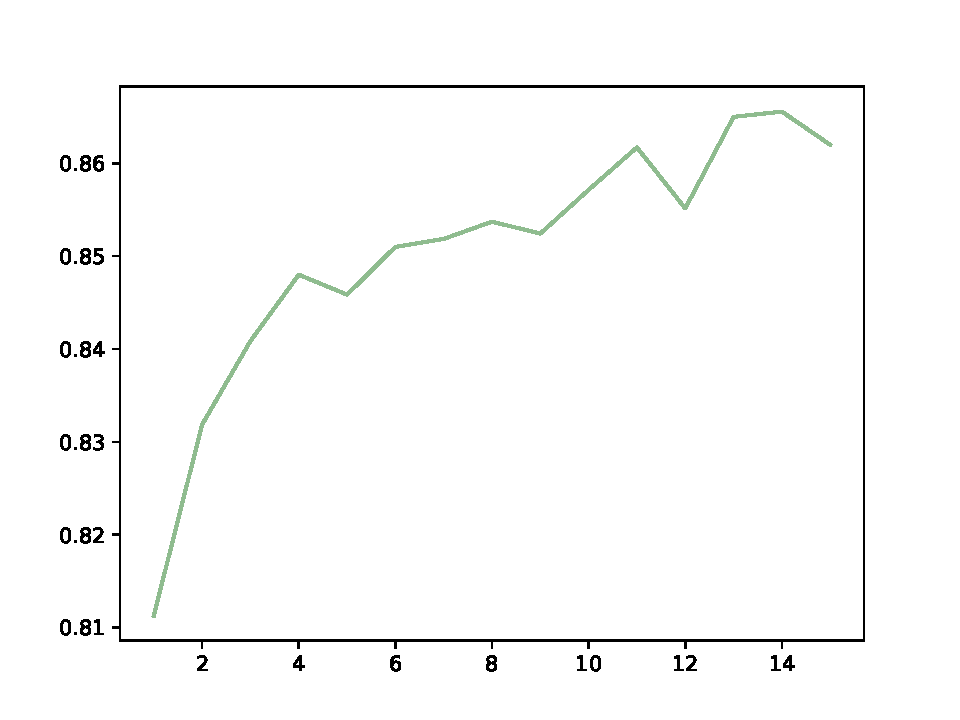
\includegraphics[scale=0.23]{imgs/test_acc_1.pdf}
  \end{minipage}
}
\caption{ train dataset : test dataset = 9 : 1}
\label{tv0.1}
\end{figure}

\begin{figure}[!h]
\subfigure[train loss ]{
  \begin{minipage}{0.21\linewidth}
  \centering
  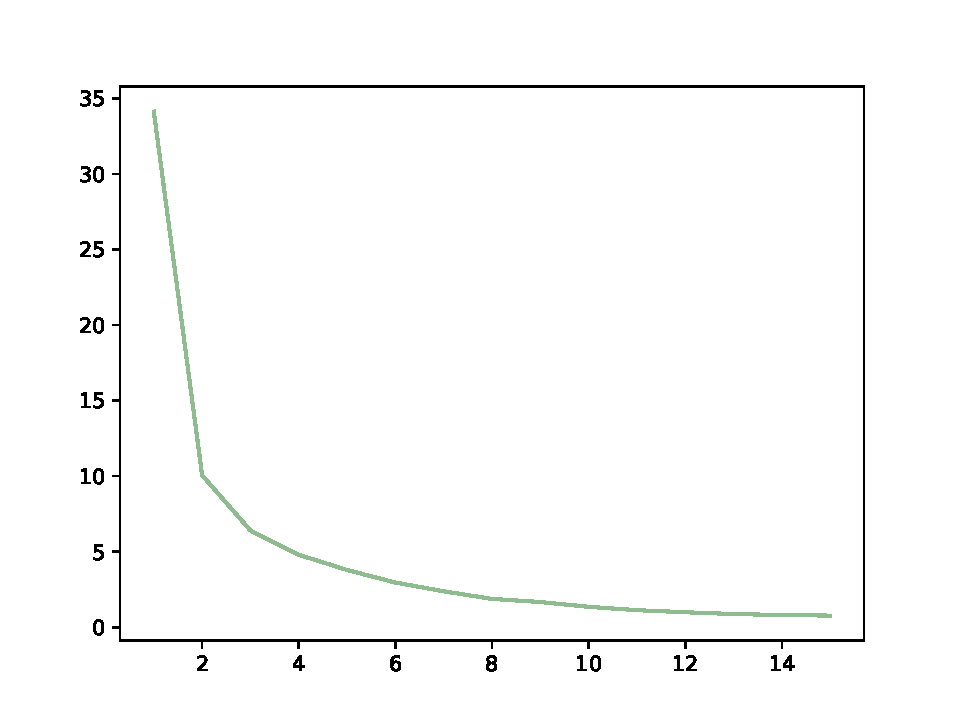
\includegraphics[scale=0.23]{imgs/train_loss_3.pdf}
  \end{minipage}
}
\quad
\subfigure[train accuracy ]{
\begin{minipage}{0.21\linewidth}
\centering
  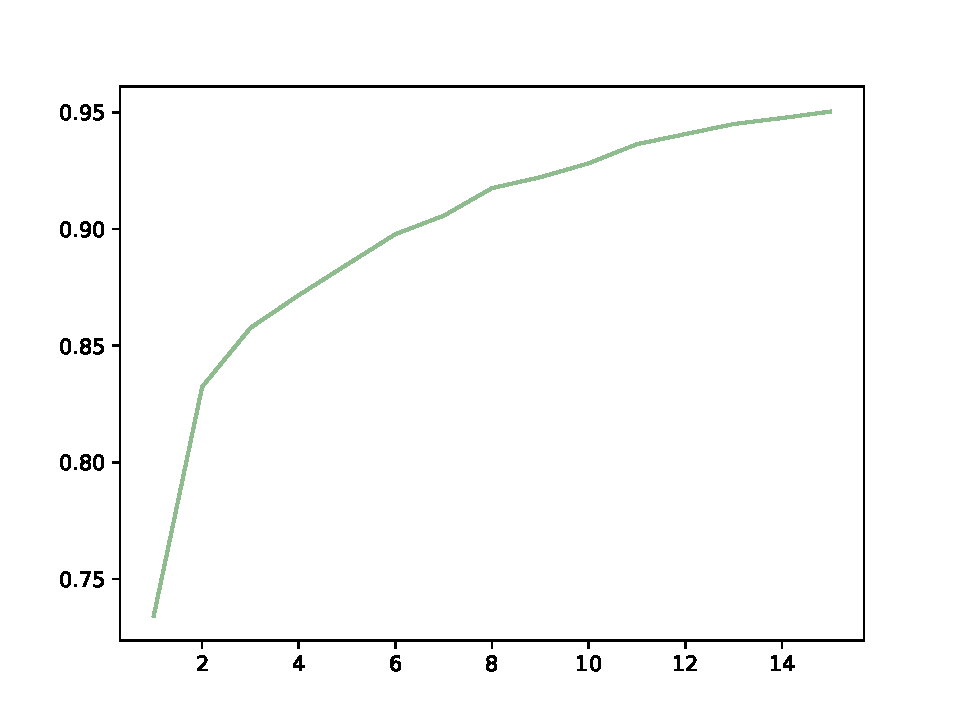
\includegraphics[scale=0.23]{imgs/train_acc_3.pdf}
  \end{minipage}
}
\quad
\subfigure[test loss ]{
\begin{minipage}{0.21\linewidth}
\centering
  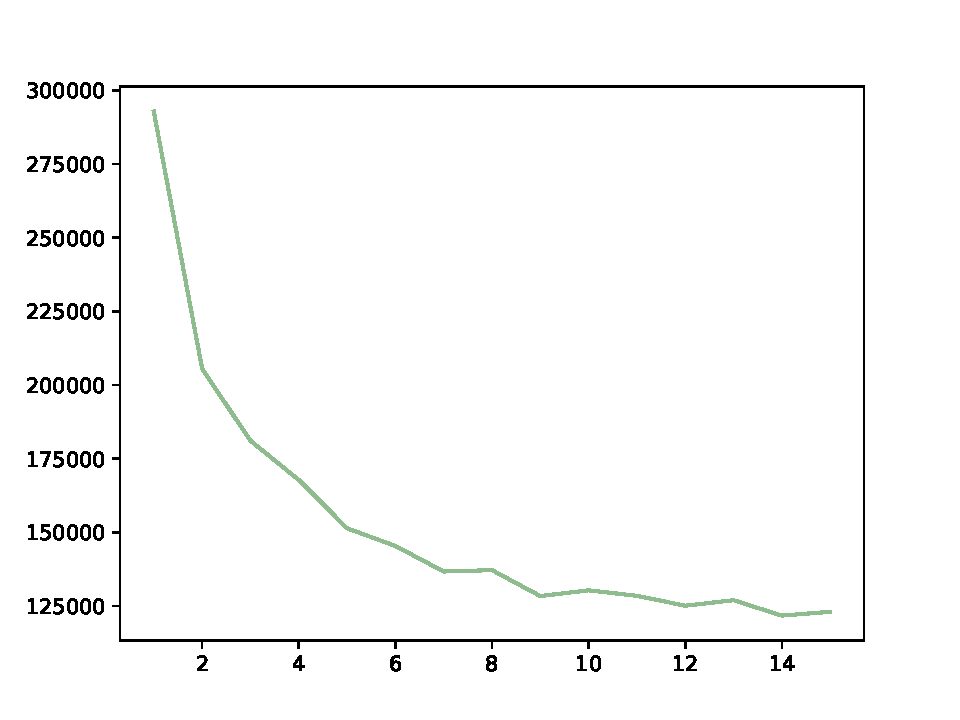
\includegraphics[scale=0.23]{imgs/test_loss_3.pdf}
  \end{minipage}
}
\quad
\subfigure[test accuracy ]{
\begin{minipage}{0.21\linewidth}
\centering
  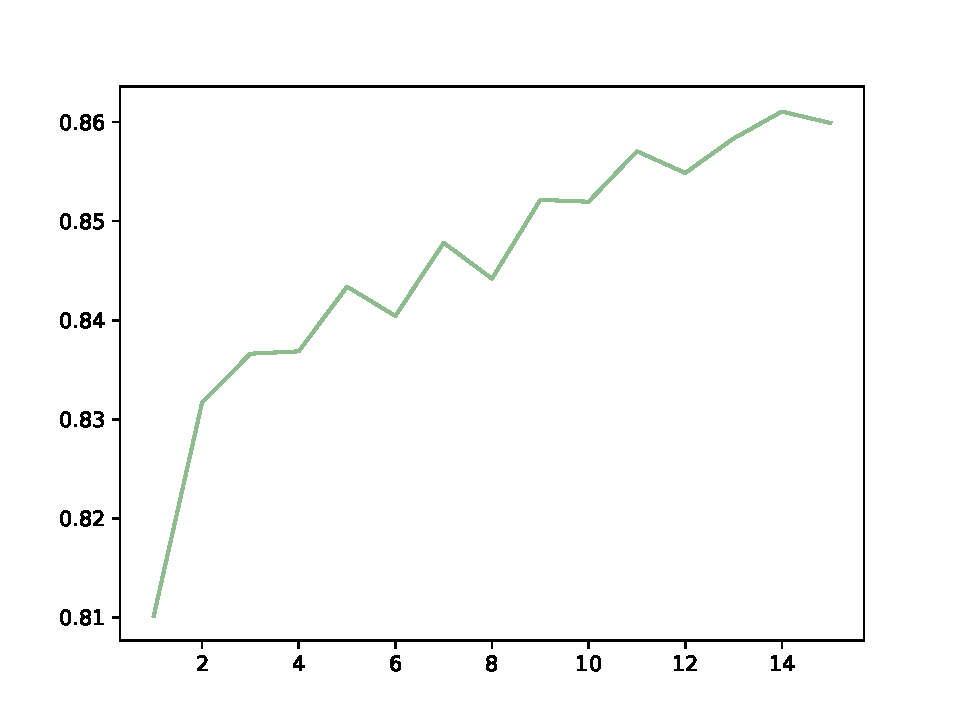
\includegraphics[scale=0.23]{imgs/test_acc_3.pdf}
  \end{minipage}
}
\caption{ train dataset : test dataset = 7 : 3}
\label{tv0.3}
\end{figure}


\begin{figure}[!h]
\subfigure[train loss ]{
  \begin{minipage}{0.21\linewidth}
  \centering
  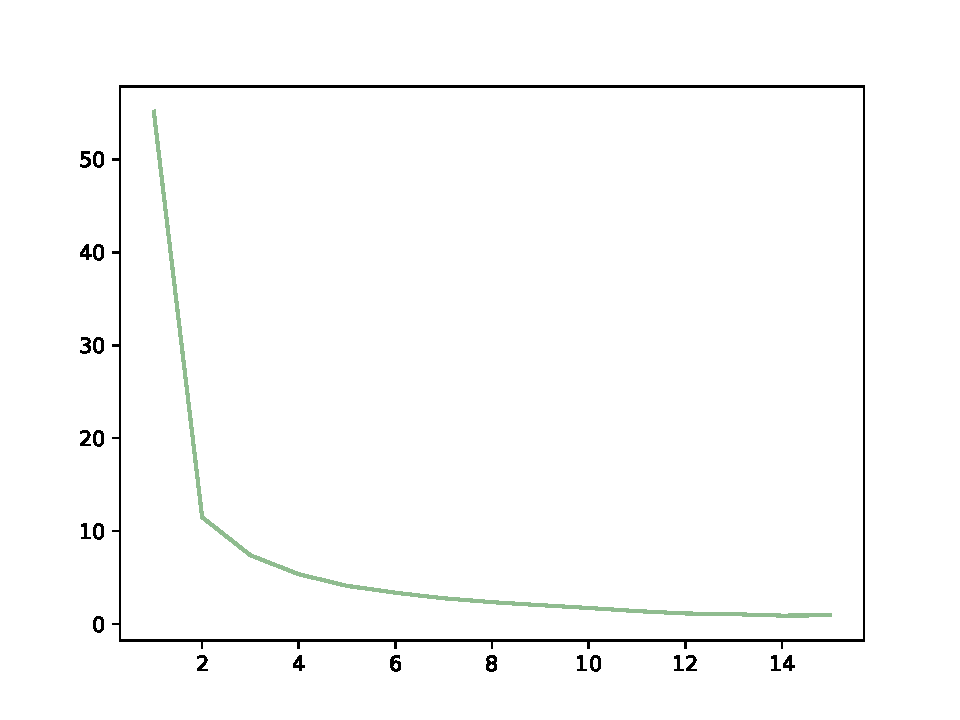
\includegraphics[scale=0.23]{imgs/train_loss_4.pdf}
  \end{minipage}
}
\quad
\subfigure[train accuracy ]{
\begin{minipage}{0.21\linewidth}
\centering
  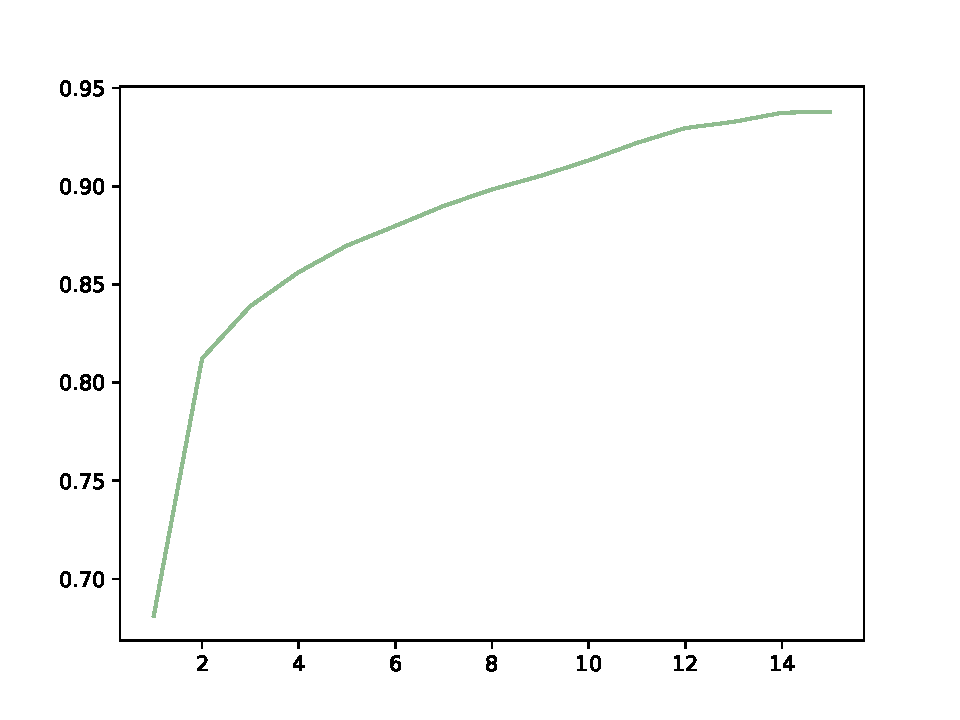
\includegraphics[scale=0.23]{imgs/train_acc_4.pdf}
  \end{minipage}
}
\quad
\subfigure[test loss ]{
\begin{minipage}{0.21\linewidth}
\centering
  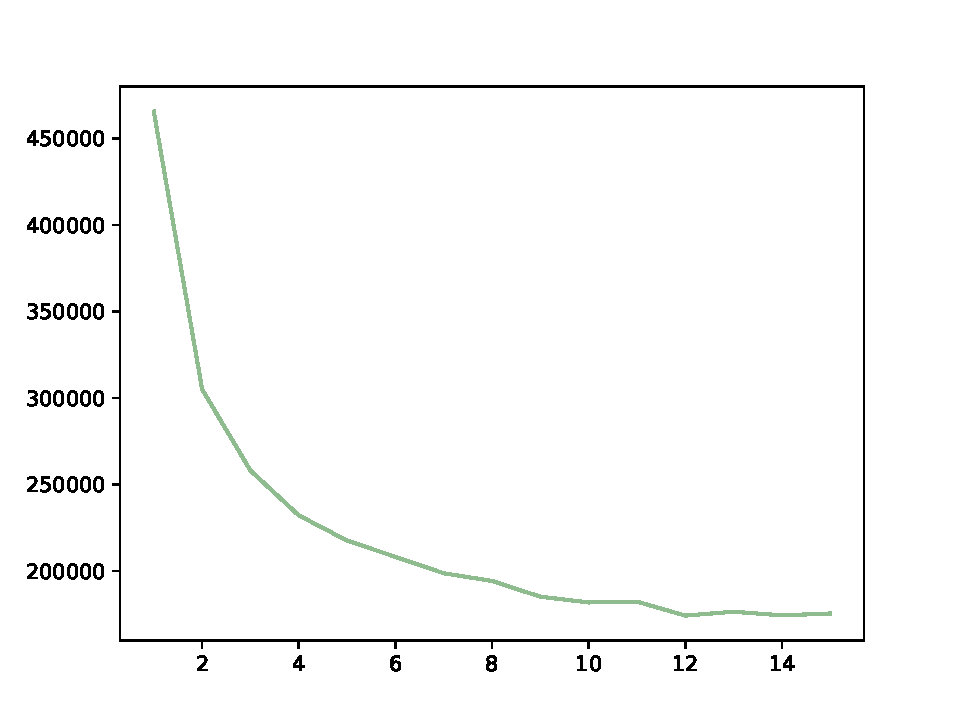
\includegraphics[scale=0.23]{imgs/test_loss_4.pdf}
  \end{minipage}
}
\quad
\subfigure[test accuracy ]{
\begin{minipage}{0.21\linewidth}
\centering
  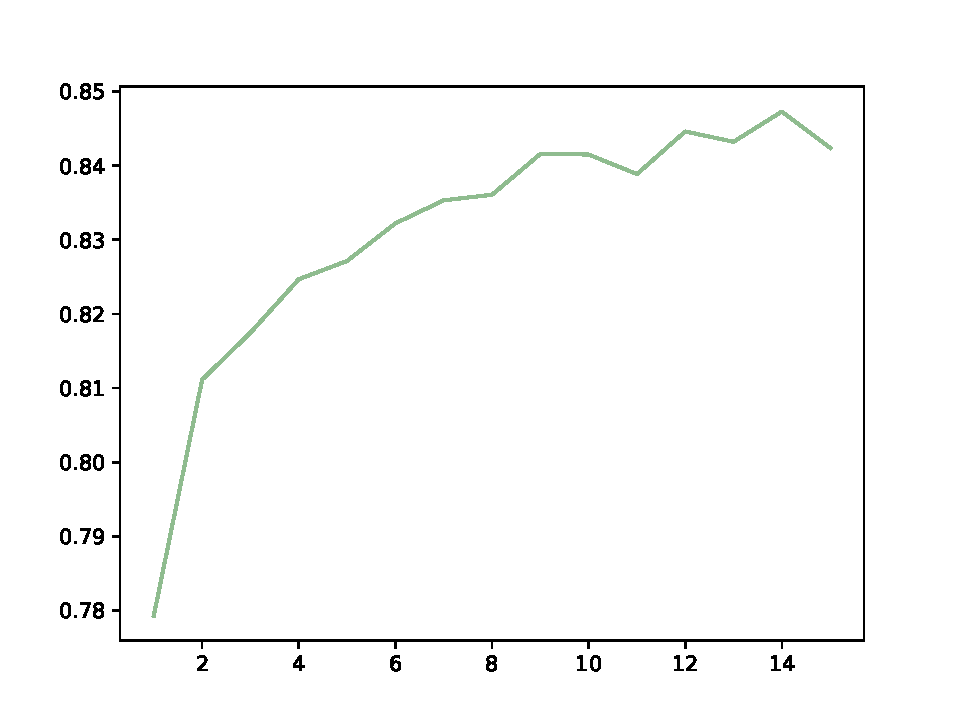
\includegraphics[scale=0.23]{imgs/test_acc_4.pdf}
  \end{minipage}
}
\caption{ train dataset : test dataset = 6 : 4}
\label{tv0.4}
\end{figure}

\subsection{Batch size}
Figure \ref{bs500} is the result of batch size 500, which can reach 86.84\% on accuracy within 15 epochs. Figure \ref{adam} is the result of batch size 1000, whose maximum of accuracy is  85.87\%. Figure \ref{bs1500} is the result of batch size 1500, whose maximum of accuracy is  85.20\%.  Batch size will affect the performance of the model. But a smaller batch size also lends to longer training time. So we need to balance those two factors based on different requirements.

\begin{figure}[!h]
\subfigure[train loss ]{
  \begin{minipage}{0.21\linewidth}
  \centering
  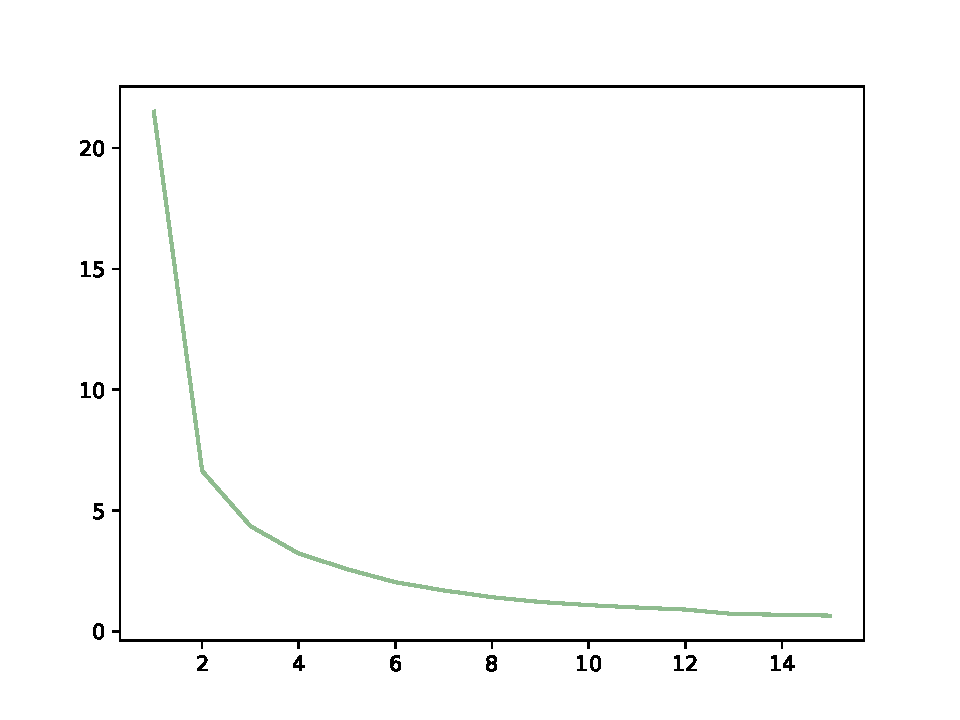
\includegraphics[scale=0.23]{imgs/train_loss_500.pdf}
  \end{minipage}
}
\quad
\subfigure[train accuracy ]{
\begin{minipage}{0.21\linewidth}
\centering
  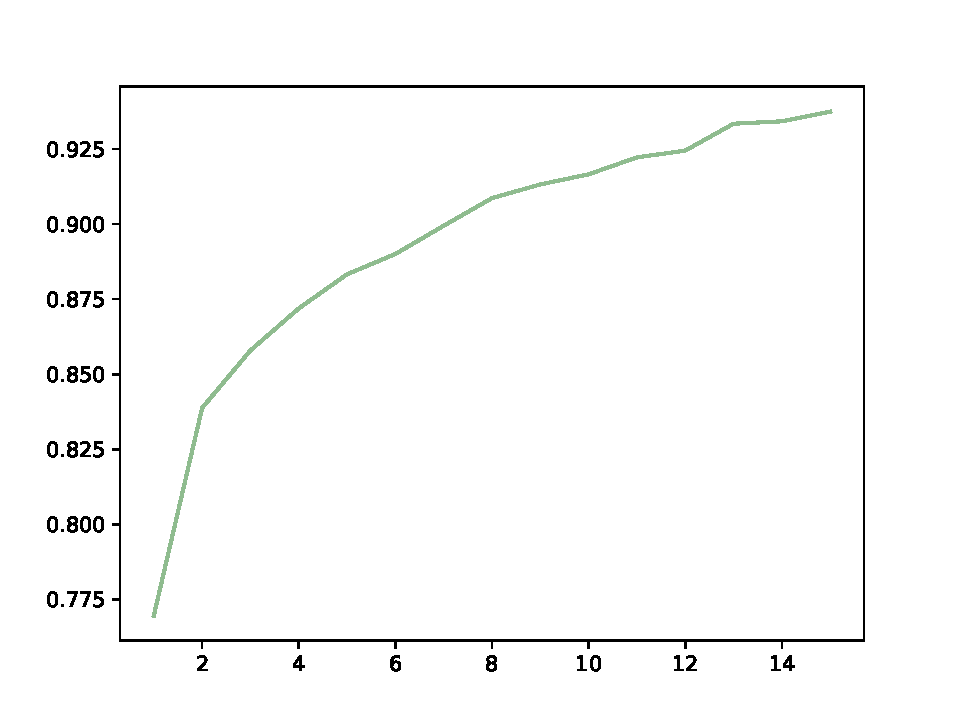
\includegraphics[scale=0.23]{imgs/train_acc_500.pdf}
  \end{minipage}
}
\quad
\subfigure[test loss ]{
\begin{minipage}{0.21\linewidth}
\centering
  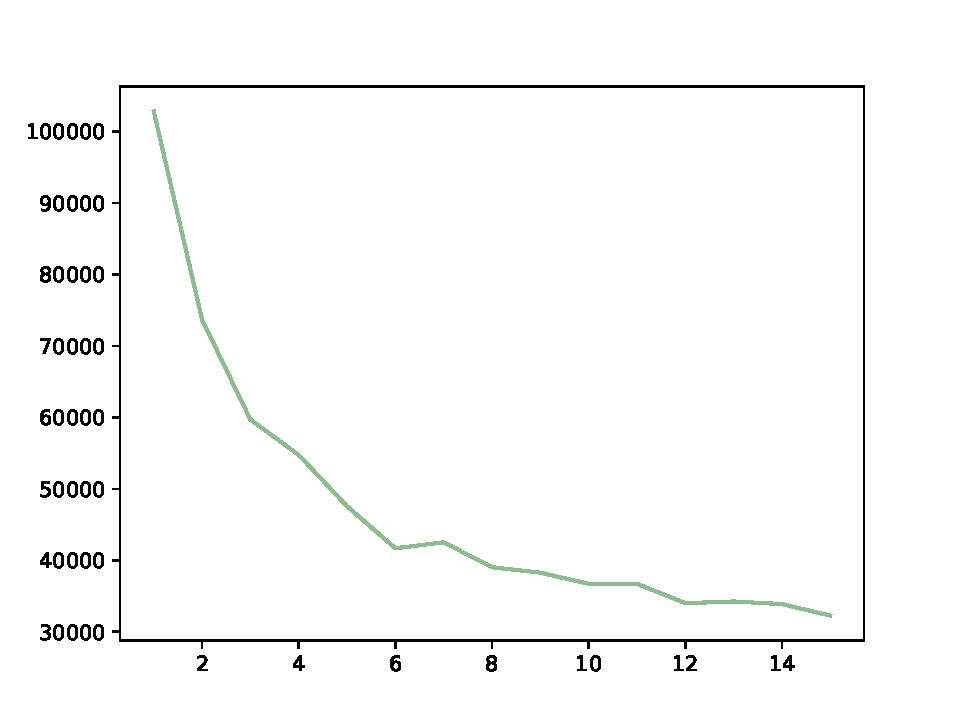
\includegraphics[scale=0.23]{imgs/test_loss_500.pdf}
  \end{minipage}
}
\quad
\subfigure[test accuracy ]{
\begin{minipage}{0.21\linewidth}
\centering
  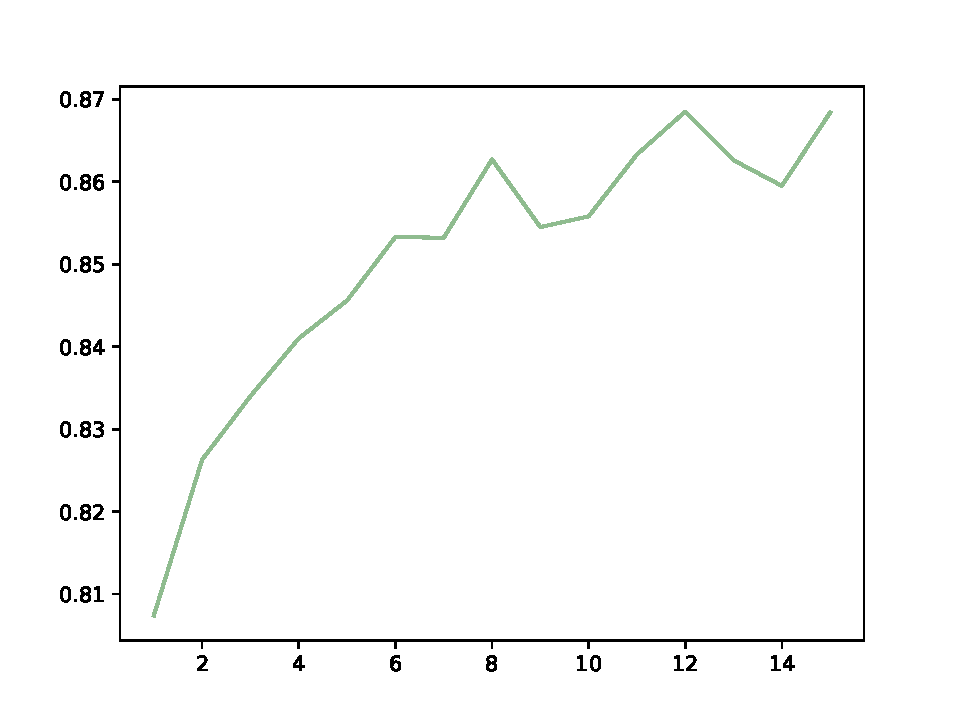
\includegraphics[scale=0.23]{imgs/test_acc_500.pdf}
  \end{minipage}
}
\caption{ Batch size: 500}
\label{bs500}
\end{figure}

\begin{figure}[!h]
\subfigure[train loss ]{
  \begin{minipage}{0.21\linewidth}
  \centering
  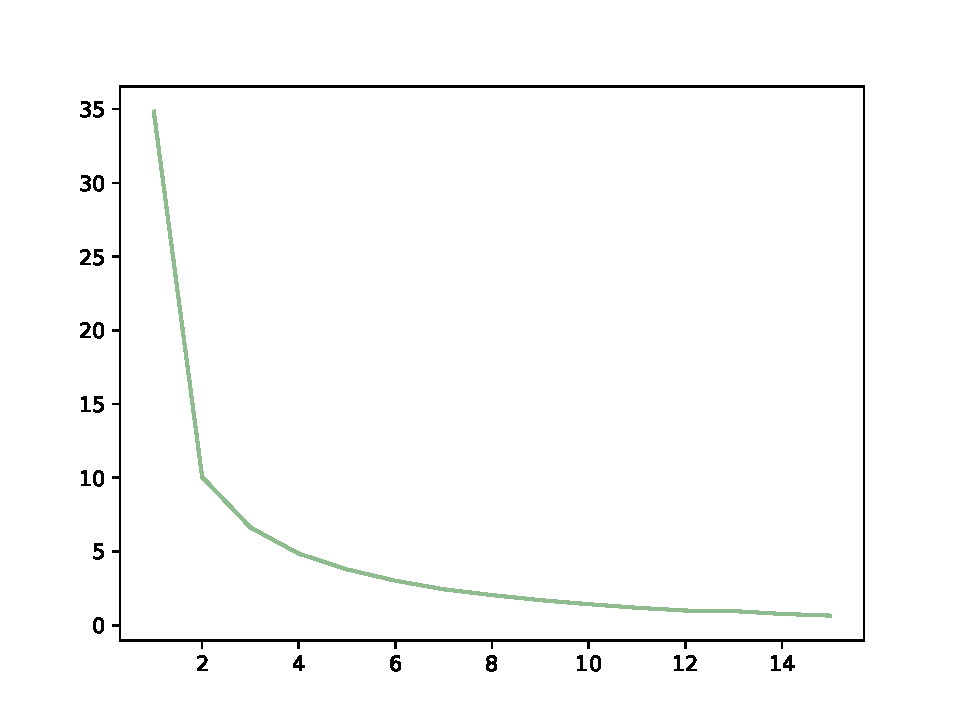
\includegraphics[scale=0.23]{imgs/train_loss_1500.pdf}
  \end{minipage}
}
\quad
\subfigure[train accuracy ]{
\begin{minipage}{0.21\linewidth}
\centering
  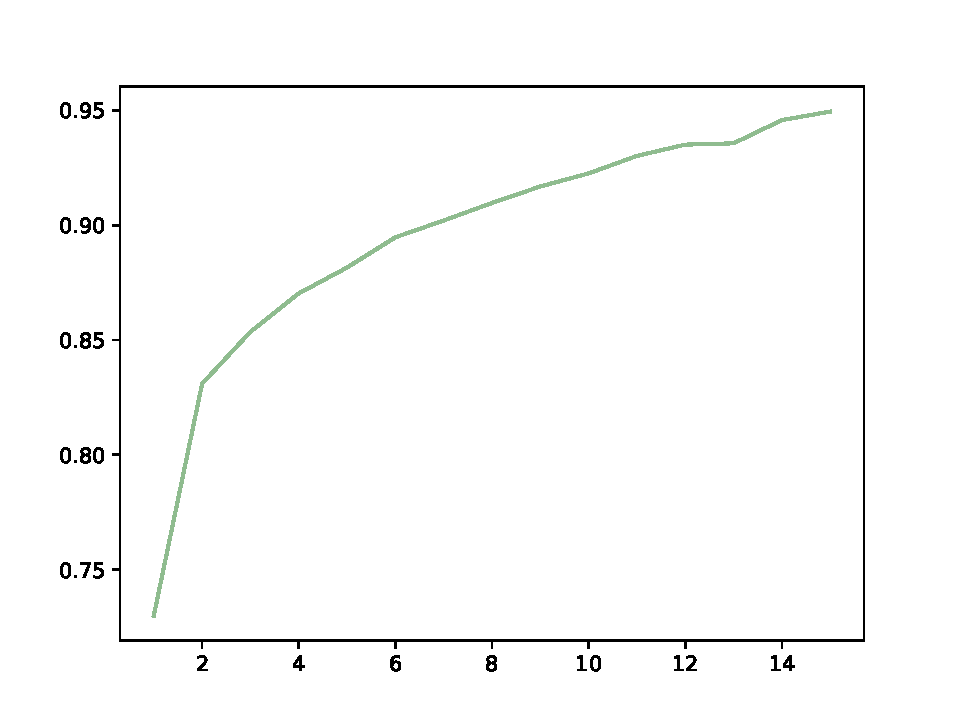
\includegraphics[scale=0.23]{imgs/train_acc_1500.pdf}
  \end{minipage}
}
\quad
\subfigure[test loss ]{
\begin{minipage}{0.21\linewidth}
\centering
  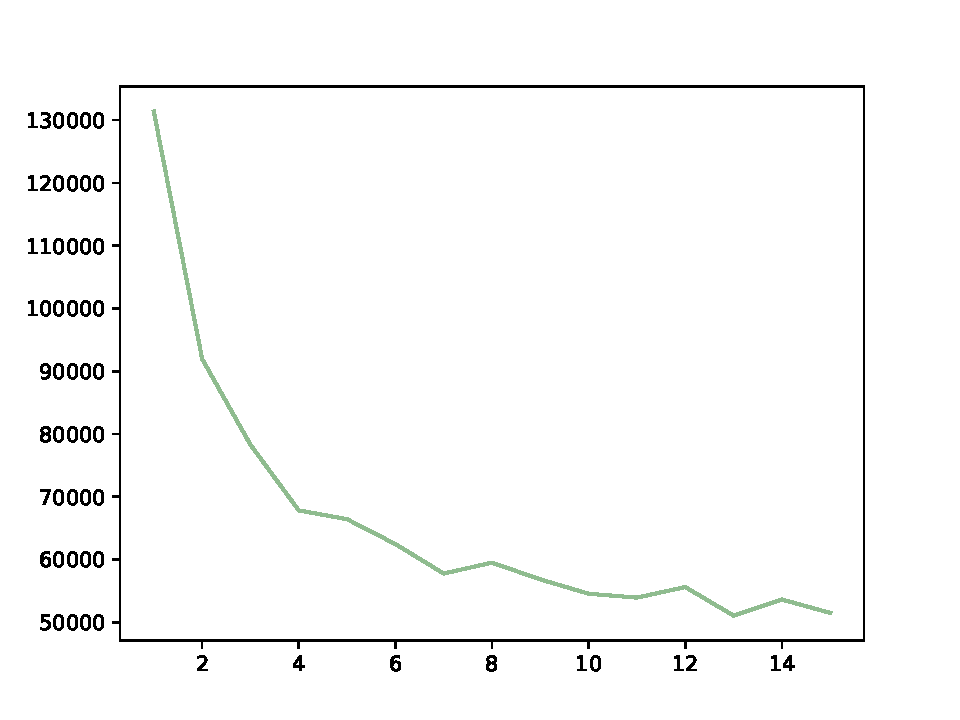
\includegraphics[scale=0.23]{imgs/test_loss_1500.pdf}
  \end{minipage}
}
\quad
\subfigure[test accuracy ]{
\begin{minipage}{0.21\linewidth}
\centering
  \includegraphics[scale=0.23]{imgs/test_acc_1500.pdf}
  \end{minipage}
}
\caption{ Batch size: 1500}
\label{bs1500}
\end{figure}

\subsection{GPU VS CPU}
I tested training time with GPU and CPU on Calab. The approximate running time of CPU per epoch is 114.79436 and of GPU is 6.03704. 

Unlike problem 1, with the model CNNs, the training time on CPU per epoch is almost 20 times than training time on GPU. 

\subsection{Overfit}
The CNNs model and Vgg16 model are not overfit according to Figure \ref{over} and  Figure \ref{vgg16}.  Normally, I'll run a model for a few epochs. If the accuracy(loss) on train dataset is very desired while those measures on the test dataset are still unreasonable, I assume the model overfits. For example, it would be a red signal if the model has 99\% accuracy on the training dataset but only 50\% accuracy on the test dataset. I'll use dropout and regularization to prevent the model overfit.


\subsection{Performance compared with other algorithms}
I tried random forest classifier(n\_estimators=100, max\_depth=30), which can achieve 87.57\% on accuracy. Decision tree algorithm could achieve 79.02\%. KNeighbors algorithm could achieve 85.54\%.

\subsection{Cluster on weights}
Because there are many weights in CNNs model, I clustered the weights from the linear model.

I tried kmeans and ksne to obtain 2 cluster as the horizontal and vertical coordinate. Figure \ref{kmean} is the result of kmeans, and Figure \ref{ksne} is the result of ksne. It's hard to see the difference in those graph.

\begin{figure}[!h]
  \centering
  \includegraphics[scale=0.5]{imgs/kmeans.png}
  \caption{KMEANS}
  \label{kmean}
\end{figure}

\begin{figure}[!h]
  \centering
  \includegraphics[scale=0.5]{imgs/ksne.png}
  \caption{KSNE}
  \label{ksne}
\end{figure}

\end{document}
